% MBDyn (C) is a multibody analysis code.
% http://www.mbdyn.org
%
% Copyright (C) 1996-2023
%
% Pierangelo Masarati  <pierangelo.masarati@polimi.it>
%
% Dipartimento di Ingegneria Aerospaziale - Politecnico di Milano
% via La Masa, 34 - 20156 Milano, Italy
% http://www.aero.polimi.it
%
% Changing this copyright notice is forbidden.
%
% This program is free software; you can redistribute it and/or modify
% it under the terms of the GNU General Public License as published by
% the Free Software Foundation (version 2 of the License).
%
%
% This program is distributed in the hope that it will be useful,
% but WITHOUT ANY WARRANTY; without even the implied warranty of
% MERCHANTABILITY or FITNESS FOR A PARTICULAR PURPOSE.  See the
% GNU General Public License for more details.
%
% You should have received a copy of the GNU General Public License
% along with this program; if not, write to the Free Software
% Foundation, Inc., 59 Temple Place, Suite 330, Boston, MA  02111-1307  USA
\emph{Author: Reinhard Resch} \\
Hydrodynamic plain bearing elements are intended to model tribological fluid-structure interactions between a bearing journal and a bearing shell.
\paragraph{Files.} \
It is implemented in files\\
\begin{tabular}{l}
  \texttt{modules/module-hydrodynamic\_plain\_bearing2/module-hydrodynamic\_plain\_bearing2.h} \\
  \texttt{modules/module-hydrodynamic\_plain\_bearing2/module-hydrodynamic\_plain\_bearing2.cc}
\end{tabular}

\section{Introduction}
Hydrodynamic lubricated journal plain bearings are used in many different types of machinery:
\begin{itemize}
\item Combustion engines
\item Turbo chargers
\item Steam turbines for power plants
\item Hydraulic pumps
\end{itemize}
MBDyn's ``module-hydrodynamic\_plain\_bearing2'' is intended to simulate the following effects in rigid or flexible multibody systems including hydrodynamic bearings:
\begin{itemize}
\item Frictional losses inside the bearing
\item Maximum contact pressure and maximum fluid pressure at the surface of the bearing
\item Minimum lubricant film thickness at the surface of the bearing
\item Demand of lubricant to be supplied by means of a hydraulic pump
\item Impact on structural damping of a mechanism due to the squeeze effect
\item Impact on stability of the orbital path for high speed and low load applications (e.g. turbo chargers)
\end{itemize}

\section{The compressible Reynolds differential equation}
\subsection{Determination of the coordinate system for the cylindrical journal bearing}
Figure~\ref{fig:h100} shows a cylindrical journal bearing with the following coordinate systems:
\begin{description}
\item[$\boldsymbol{R}_{b1}$] Coordinate system in the center of the bearing journal
\item[$\boldsymbol{R}_{b2}$] Coordinate system in the center of the bearing shell
\item[$\boldsymbol{R}_{t1}$] Coordinate system tangential to the surface of the bearing journal
\item[$\boldsymbol{R}_{t2}$] Coordinate system tangential to the surface of the bearing shell
\end{description}
The following symbols are used:
\begin{description}
\item[$R$] Radius of the bearing shell
\item[$r$] Radius of the bearing journal
\item[$B$] Width of the bearing shell or bearing journal
\item[$h$] Radial radial gap height
\end{description}

\begin{figure}[htb]
\centering
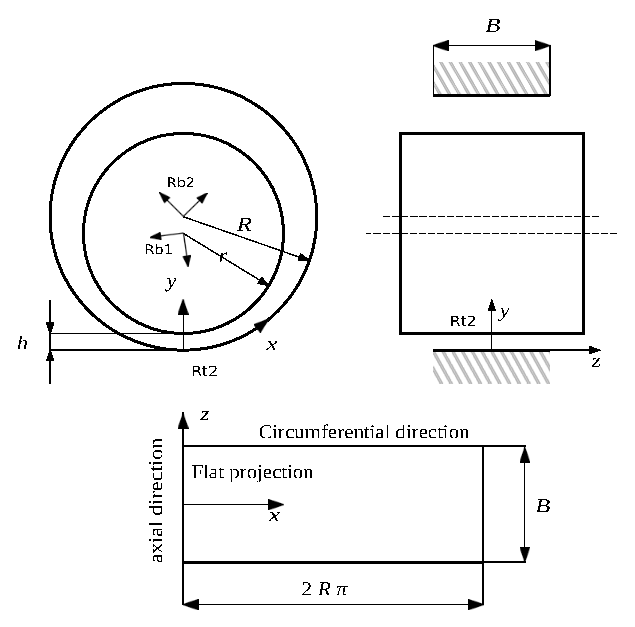
\includegraphics[width=0.5\linewidth]{fig_h100en}
\caption{Coordinate systems for cylindrical plain bearings}
\label{fig:h100}
\end{figure}

The $z$~axes of $\boldsymbol{R}_{b1}$ and $\boldsymbol{R}_{b2}$ correspond to the axes of the bearing journal and bearing shell. The $x$ and $y$~axis can be defined as required. The $x$~axis of $\boldsymbol{R}_{t2}$ is tangential to the circumference of the bearing shell, the $y$~axis is in the radial direction and the $z$~axis is parallel to the $z$~axis of $\boldsymbol{R}_{b2}$. The derivation of the Reynolds differential equation in section~\ref{sec:navier_stokes} is based on the coordinate system~$\boldsymbol{R}_{t2}$. However, $\boldsymbol{R}_{t1}$ could just as well be used.

\subsection{Derivation of the Reynolds equation from the compressible Navier Stokes equation}
\label{sec:navier_stokes}
Since, according to \cite{Butenschoen-1976}, the radial gap height $h$ is small compared to the radius $R$, the curvature of the oil-filled gap can be neglected. For this reason, as shown in Figure~\ref{fig:h100}, the volume of the gap can be unrolled onto a plane and the Navier Stokes equation can be written in Cartesian coordinates. If we assume a Newtonian fluid with constant viscosity and laminar flow, then according to \cite{DIRKBARTEL2010} the Navier Stokes equation given in equation~\ref{eq:h100} follows for the flow in $x$ and $z$~direction. As the flow velocity in the radial gap height direction is neglected, the Navier Stokes equation for the $y$~direction is not applicable.

\begin{IEEEeqnarray}{rCl}
\label{eq:h100}
\underbrace{\rho\,\left(\frac{\partial u_x}{\partial t} + u_x \, \frac{\partial u_x}{\partial x} + u_y \, \frac{\partial u_x}{\partial y} + u_z \, \frac{\partial u_x}{\partial z} \right)}_{\approx 0}&=&\underbrace{\rho\,g_x}_{\approx 0}-\frac{\partial p}{\partial x}+\underbrace{2\,\eta\,\frac{\partial^2 u_x}{\partial x^ 2}}_{\approx 0}-\frac{2}{3}\,\eta\,\left(\underbrace{\frac{\partial^2 u_x}{\partial x^2}}_{\approx 0}+\underbrace{\frac{\partial^2 u_y}{\partial x\,\partial y}}_{\approx 0} + \underbrace{\frac{\partial^2 u_z}{\partial x\,\partial z}}_{\approx 0}\right) \nonumber \\
&&+\eta\,\left(\frac{\partial^2 u_x}{\partial y^2} + \underbrace{\frac{\partial^2 u_y}{\partial x\,\partial y}}_{\approx 0}\right)+\eta\,\left(\underbrace{\frac{\partial^2 u_x}{\partial z^2}}_{\approx 0} + \underbrace{\frac{\partial^2 u_z}{\partial x\,\partial z}}_{\approx 0}\right) \nonumber \\
\underbrace{\rho\,\left(\frac{\partial u_z}{\partial t} + u_x \, \frac{\partial u_z}{\partial x} + u_y \, \frac{\partial u_z}{\partial y} + u_z \, \frac{\partial u_z}{\partial z}\right)}_{\approx 0}&=&\underbrace{\rho\,g_z}_{\approx 0}-\frac{\partial p}{\partial z}+\underbrace{2\,\eta\,\frac{\partial^2 u_z}{\partial z^2}}_{\approx 0}-\frac{2}{3}\,\eta\,\left(\underbrace{\frac{\partial^2 u_x}{\partial x\,\partial z}}_{\approx 0}+\underbrace{\frac{\partial^2 u_y}{\partial y\,\partial z}}_{\approx 0} + \underbrace{\frac{\partial^2 u_z}{\partial z^2}}_{\approx 0}\right) \nonumber \\
&&+\eta\,\left(\underbrace{\frac{\partial^2 u_x}{\partial x\,\partial z}}_{\approx 0} + \underbrace{\frac{\partial^2 u_z}{\partial x^2}}_{\approx 0}\right)+\eta\,\left(\underbrace{\frac{\partial^2 u_y}{\partial y\,\partial z}}_{\approx 0} + \frac{\partial^2 u_z}{\partial y^2}\right)
\end{IEEEeqnarray}

\begin{description}
\item[$\boldsymbol{u}=\begin{pmatrix} u_x \cr u_z \end{pmatrix}$] Flow velocity measured in the coordinate system $\boldsymbol{R}_{t1}$ or $\boldsymbol{R}_{t2}$\footnote{Strictly speaking, an inertial coordinate system would have to be used for the derivation. However, since the inertial forces are neglected in the derivation of Reynolds' differential equation, this does not matter}
\item[$p$] Pressure
\item[$\rho$] Density
\item[$\eta$] dynamic viscosity
\end{description}

According to \cite{Butenschoen-1976} and \cite{DIRKBARTEL2010}, the following simplifying assumptions can be made:
\begin{itemize}
\item Due to the small Reynolds numbers present in hydrodynamic plain bearings, the inertia forces can be neglected compared to the pressure forces and the frictional forces.
\item The gravity loads can also be neglected compared to the pressure forces and the frictional forces.
\item Since the radial gap height $h$ is very small compared to the bearing width $B$ and the bearing circumference $2\,R\,\pi$ for the usual bearing dimensions, the velocity gradients in $x$ and $z$~direction can be neglected in the friction terms compared to the velocity gradients in $y$ direction.
\item It is also assumed that the pressure change in the direction of the radial gap height is negligible. For the same reason, the Navier Stokes equation for the $y$ direction is also omitted.
\end{itemize}
With these assumptions, equation~\ref{eq:h100} is reduced to equation~\ref{eq:h200}.


\begin{IEEEeqnarray}{rCl}
\label{eq:h200}
\frac{\partial p}{\partial x} & = & \eta \, \frac{\partial^2 u_x}{\partial y^2} \nonumber \\
\frac{\partial p}{\partial z} & = & \eta \, \frac{\partial^2 u_z}{\partial y^2}
\end{IEEEeqnarray}

\subsubsection{Boundary conditions for the flow velocity at the bearing surface}
If it is assumed that the fluid adheres to the surface of the bearing journal and the surface of the bearing shell, the boundary conditions according to equation~\ref{eq:h300} apply\cite{Butenschoen-1976}. This requirement is usually fulfilled for radial plain bearings by selecting the appropriate bearing materials, as the adhesion condition is of decisive importance for the load carrying capacity of the bearing. For piston-cylinder bearings, however, adhesion to the surface is not absolutely necessary. For example, when using special coatings for pistons, the adhesion condition may not be fulfilled. However, this case is excluded here.
\begin{IEEEeqnarray}{rCl}
\label{eq:h300}
\left. u_x \right\vert_{y=0}&=& \Delta U_{2x} \nonumber \\
\left. u_x \right\vert_{y=h}&=& \Delta U_{1x} \nonumber \\
\left. u_z \right\vert_{y=0}&=& \Delta U_{2z} \nonumber \\
\left. u_z \right\vert_{y=h}&=& \Delta U_{1z}
\end{IEEEeqnarray}

When introducing the boundary conditions, care must be taken to ensure that they are objective. A distinction is made between two cases:
\subparagraph{control volume moves with the bearing journal}
\begin{IEEEeqnarray}{rCl}
\Delta\boldsymbol{U}_1&=&\boldsymbol{0} \\
\Delta\boldsymbol{U}_2&=&\boldsymbol{U}_2 - \boldsymbol{U}_1
\end{IEEEeqnarray}

\subparagraph{control volume moves with the bearing shell}
\begin{IEEEeqnarray}{rCl}
\Delta\boldsymbol{U}_1&=&\boldsymbol{U}_1 - \boldsymbol{U}_2 \\
\Delta\boldsymbol{U}_2&=&\boldsymbol{0}
\end{IEEEeqnarray}

Obviously, the boundary conditions depend on the choice of control volume. However, the derivation of the radial gap height $\frac{\partial h}{\partial t}$ also depends on the choice of control volume. The kinematic relationships are discussed in section~\ref{sec:h100}.

\begin{description}
\item[$\boldsymbol{U}_1$] Absolute velocity at the surface of the bearing journal projected into the coordinate system $\boldsymbol{R}_{t1}$ or $\boldsymbol{R}_{t2}$
\item[$\boldsymbol{U}_2$] Absolute velocity at the surface of the bearing shell projected into the coordinate system $\boldsymbol{R}_{t1}$ or $\boldsymbol{R}_{t2}$
\item[$\Delta\boldsymbol{U}_1=\begin{pmatrix} \Delta U_{1x} \cr \Delta U_{1y} \cr \Delta U_{1z} \end{pmatrix}$] Velocity of the surface of the bearing journal relative to the control volume
\item[$\Delta\boldsymbol{U}_2=\begin{pmatrix} \Delta U_{2x} \cr \Delta U_{2y} \cr \Delta U_{2z} \end{pmatrix}$] Velocity of the surface of the bearing shell relative to the control volume
\end{description}

If equation~\ref{eq:h200} is integrated twice over the radial gap height and the boundary conditions \ref{eq:h300} are used, this results in a parabolic velocity distribution in the direction of the radial gap height\cite{Butenschoen-1976}, \cite{DIRKBARTEL2010}.
\begin{IEEEeqnarray}{rCl}
u_x&=&\frac{1}{\eta}\,\frac{\partial p}{\partial x}\,\left(\frac{y^2}{2} - y\,\frac{h}{2}\right) + \frac{\Delta U_{1x} - \Delta U_{2x}}{h}\,y + \Delta U_{2x} \nonumber \\
u_z&=&\frac{1}{\eta}\,\frac{\partial p}{\partial z}\,\left(\frac{y^2}{2} - y\,\frac{h}{2}\right) + \frac{\Delta U_{1z} - \Delta U_{2z}}{h}\,y + \Delta U_{2z}
\label{eq:h325}
\end{IEEEeqnarray}

For the mass flow per unit length through the edges of the control volume, the following applies\cite{Butenschoen-1976}, \cite{DIRKBARTEL2010}
\begin{IEEEeqnarray}{rClrCl}
\dot{m}_x & = & \int_{y=0}^{y=h} \rho\,u_x\,dy & = & \rho \, \underbrace{\int_{y=0}^{y=h} u_x \,
dy}_{q_x}
\\
\dot{m}_z & = & \int_{y=0}^{y=h} \rho\,u_z\,dy & = & \rho \, \underbrace{\int_{y=0}^{y=h}
\,u_z\,dy}_{q_z}
\end{IEEEeqnarray}

It is assumed in this work that the density $\rho$ is only a function of the pressure $p$. Since the pressure is assumed to be constant in the direction of the radial gap height, the density is also constant in the $y$~direction.

\begin{IEEEeqnarray}{rCl}
\dot{m}_x&=&\rho \, q_x \\
\dot{m}_z&=&\rho \, q_z \\
q_x &=& \underbrace{\frac{\Delta U_{1x} + \Delta U_{2x}}{2}\,h}_{\text{Couette fraction}}
                \underbrace{- \frac{h^3}{12\,\eta}\,\frac{\partial p}{\partial x}}_{\text{Poiseuille fraction}} \\
q_z & = & \underbrace{\frac{\Delta U_{1z} + \Delta U_{2z}}{2}\,h}_{\text{Couette fraction}}
                  \underbrace{- \frac{h^3}{12\,\eta}\,\frac{\partial p}{\partial z}}_{\text{Poiseuille fraction}}
\end{IEEEeqnarray}

The compressible Reynolds differential equation~\ref{eq:h350} follows from the application of the continuity equation to the infinitesimal volume element\cite{Butenschoen-1976}, \cite{DIRKBARTEL2010}. To close this equation, a relationship between pressure and density must be specified. This is the task of the cavitation model.
\begin{IEEEeqnarray}{rCl}
\label{eq:h350}
\underbrace{\frac{\partial}{\partial t}\left(\rho \, h\right)}_{a} & = & -\frac{\partial \dot{m}_x}{\partial x} -\frac{\partial \dot{m}_z}{\partial z} \nonumber \\
&=&-\frac{\partial}{\partial x} \, \left[\rho \, \left(\frac{\Delta U_{1x} + \Delta U_{2x}}{2} \, h - \frac{h^3}{12 \, \eta} \, \frac{\partial p}{\partial x} \right) \right] \nonumber \\
&&-\frac{\partial}{\partial z} \, \left[ \rho \, \left(\frac{\Delta U_{1z} + \Delta U_{2z}}{2} \, h - \frac{h^3}{12 \, \eta} \, \frac{\partial p}{\partial z} \right) \right]
\end{IEEEeqnarray}

\section{Cavitation models}
\subsection{Non-mass conserving cavitation}
\subsubsection{The incompressible Reynolds differential equation}
For the incompressible case, the density $\rho$ is constant. This results in a linear partial differential equation of elliptic type with the pressure $p$ as an unknown.
\begin{IEEEeqnarray}{rCl}
\frac{\partial q_x}{\partial x} + \frac{\partial q_z}{\partial z} + \frac{\partial h}{\partial t} & = &
\frac{\partial}{\partial x}\left(\frac{\Delta U_{1x} + \Delta
U_{2x}}{2}\,h-\frac{h^3}{12\,\eta}\,\frac{\partial p}{\partial x}\right) \nonumber \\
&&+\frac{\partial}{\partial z}\left(\frac{\Delta U_{1z} + \Delta U_{2z}}{2}\,h -
\frac{h^3}{12\,\eta}\,\frac{\partial p}{\partial z}\right) + \frac{\partial h}{\partial t} = 0
\end{IEEEeqnarray}
\subsubsection{The G\"umbel boundary condition}
After discretization using finite differences or finite elements, a linear system of equations results. Since no cavitation model was used, its solution can contain negative pressures\cite{Butenschoen-1976}. According to \cite{Butenschoen-1976}, the negative pressures are set to zero after the solution of the linear system of equations in accordance with the G\"umbel boundary condition. However, this violates the continuity equation at the edge of the cavitation region. According to \cite{Butenschoen-1976}, this causes an error in the pressure distribution. That error is increasing with the pressure gradient. The analytical solution of the incompressible Reynolds differential equation for an infinitely wide bearing given in \cite{Butenschoen-1976} results in a deviation in the Sommerfeld number between G\"umbel boundary condition and Reynolds boundary condition of $18\%$ with a relative eccentricity of $\varepsilon=0.999$ for the case of pure rotary motion\cite{Butenschoen-1976}. See also Figure~\ref{fig:h300}. Due to its simple implementation, the G\"umbel boundary condition was used for the incompressible case. With this method, however, it is not possible to calculate the amount of oil supplied via a lubrication groove as soon as the G\"umbel boundary condition becomes active, as the global mass conservation is not fulfilled. Instead, the required oil quantity must be calculated from the volume flow that exits via the bearing edges.

\begin{figure}[htb]
\centering
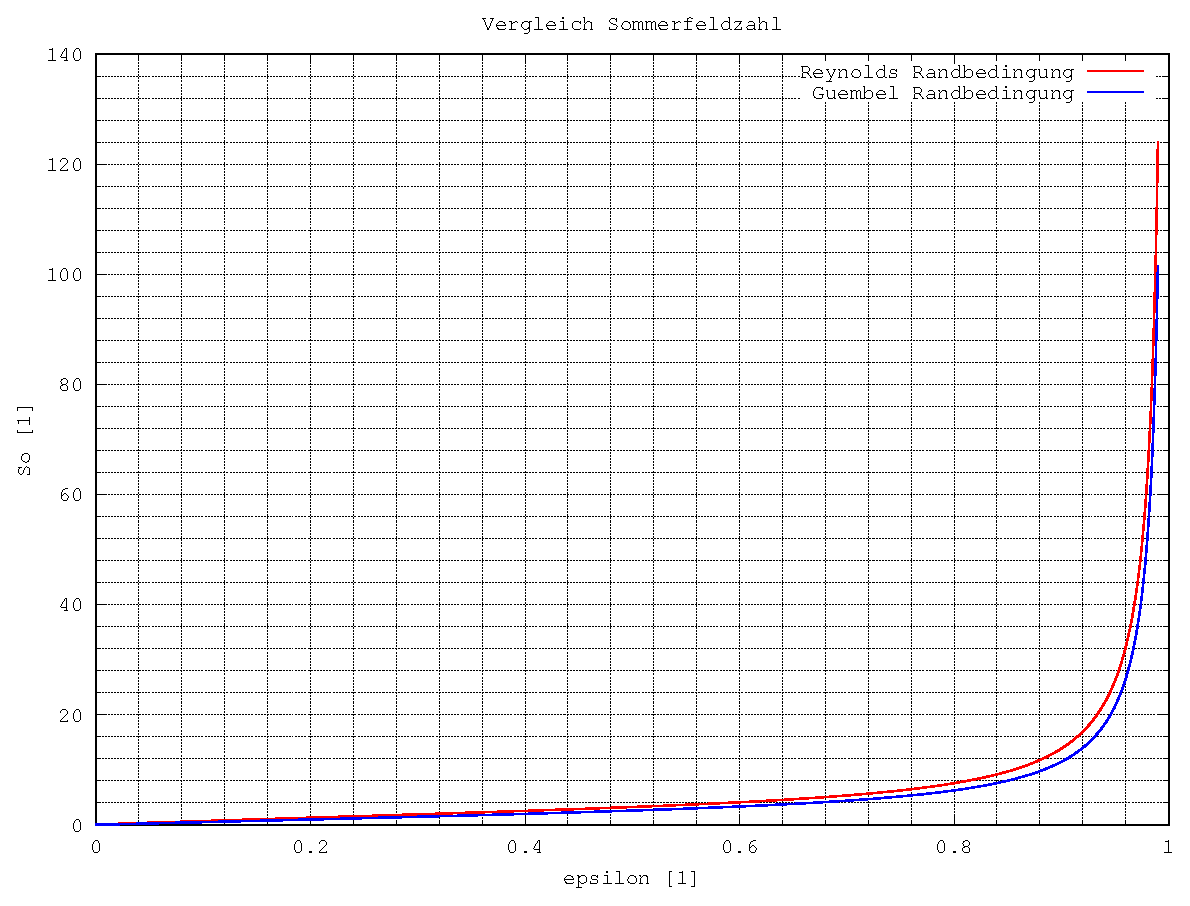
\includegraphics[width=0.5\linewidth]{fig_h300}
\caption[Differences between Reynolds boundary condition and G\"umbel boundary condition]{Differences in the Sommerfeld number between the Reynolds boundary condition and the G\"umbel boundary condition for the infinitely wide bearing with pure rotary motion}
\label{fig:h300}
\end{figure}

\subsubsection{The Reynolds boundary condition}
According to \cite{Butenschoen-1976}, the Reynolds boundary condition also requires that the pressure gradient is zero where the pressure is also zero. As a result, the continuity equation according to \cite{Butenschoen-1976} is fulfilled at least at the edge of the cavitation region. In the cavitation region itself, however, the continuity equation is still not fulfilled according to \cite{DIRKBARTEL2010}. The implementation of the Reynolds boundary condition is much more difficult than the implementation of the G\"umbel boundary condition. In \cite{Butenschoen-1976}, for example, the pressures in the widest gap were iteratively adjusted to fulfill the Reynolds boundary condition. However, this method is only applicable in the case of a pure rotary motion. According to \cite{Bayada-2013}, it is possible to obtain the Reynolds boundary condition for the general case by setting the negative pressures to zero during the iterative solution of the linear system of equations using the Gauss Seidel method. However, this method only works if the matrices of the linear system of equations are symmetrically positive definite. As this is not the case in the multi-body system used, this method could not be implemented there. For test purposes, however, this method was implemented in a stand-alone finite element program for the solution of the incompressible Reynolds equation.

\subsection{Mass conserving cavitation}
\subsubsection{The Jakobsson Floberg Ollson (JFO) cavitation model}
According to \cite{Elrod-1981}, the so-called JFO cavitation model assumes that the flow in the cavitation region is divided into oil-filled strips and strips with oil vapor or dissolved gas. It is assumed that in the oil-filled strips the radial gap height is completely filled with oil. In the cavitation region where the mean density is less than the density of the liquid oil, the vapor pressure $p_c$ is uniform. This means that only Couette flow is possible in this region. In the full-film region where the pressure is greater than $p_c$, the fluid is assumed to be incompressible. The implementation of the JFO model is relatively complex as the edges of the cavitation region must be treated explicitly.
\subsubsection{The cavitation model of H. G. Elrod}
In \cite{Elrod-1981}, Elrod assumes in contrast to the JFO theory that the fluid in the full-film region is linearly compressible. The pressure is represented as a function of density.
\begin{IEEEeqnarray}{rCl}
p&=&p_c + g \, \beta \, \left(\Theta - 1\right) \nonumber \\
g & = & \left\{
\begin{array}{rcl}
1 & \text{if} & \Theta \geq 1 \\
0 & \text{if} & \Theta < 1
\end{array}
\right. \\
\Theta & = & \frac{\rho}{\rho_c}
\label{eq:h400}
\end{IEEEeqnarray}

\begin{description}
\item[$p_c$] Cavitation pressure
\item[$\rho_c$] Cavitation density
\item[$\beta$] bulk modulus
\item[$\Theta$] dimensionless density/pressure
\end{description}

By assuming a slightly compressible fluid, it is possible to calculate the distribution of pressure and density in the bearing without having to know the edges of the cavitation region. The problem is that the bulk modulus $\beta$ is very high, which affects the numerical stability. According to \cite{Luis-San-Andres-2010}, for example, the bulk modulus of mineral oil is $\beta=2.41GPa$. To avoid numerical stability problems, \cite{Luis-San-Andres-2010} often uses values for $\beta$ that are ten to one hundred times smaller than the physically correct bulk modulus. This circumstance was taken into account in \cite{Elrod-1981} by assuming the fluid to be incompressible for the calculation of the mass flows. The linear compressibility of the fluid is only taken into account in the term $a$ in equation~\ref{eq:h350}. According to \cite{Francisco-2009}, this makes it possible to artificially reduce the bulk modulus $\beta$ without affecting the results for the steady state. According to \cite{Francisco-2009}, the choice of the bulk modulus only influences the rate of convergence with which the solution tends towards the steady state. However, a reduction of $\beta$ is not applicable to transient analysis at all, because the orbital path would be affected for sure.

\paragraph{The solution of the cavitation condition based on a mixed-complementarity problem}
Since the original Elrod model is not really applicable, it is necessary to modify the solution procedure. Instead of having only one unknown variable (e.g. either pressure $p$ or density $\rho$), it is necessary to solve for $p$ and $rho$ simultaneously, and to add another inequality in order to make the mathematical problem well posed.
Now the complementarity condition describing the cavitation model is:
\begin{itemize}
\item If $p \geq 0$ then $\rho = \rho_{liquid}$
\item If $\rho$ < $\rho_{liquid}$ then $p = 0$
\end{itemize}
Where $\rho_{liquid}$ is a constant value which is the density of pure liquid without void fraction. Actually $\rho >= 0$ is not a complementary condition but usually it is not hard to fulfill. In any case, it is necessary to use a dedicated nonlinear solver like \href{https://github.com/siconos/siconos}{SICONOS}, for the solution of this so called mixed-nonlinear complementarity problem.

\section{Discretization of the Reynolds differential equation using finite differences}
\label{sec:h150}
\subsection{The orthogonal finite difference mesh of a cylindrical journal bearing}
Figure~\ref{fig:h150} shows the basic structure of such a mesh. The grid spacing does not have to be equidistant. For example, it is possible to refine the mesh in the areas of the piston skirt and the sealing edge of the piston. To make it easier to implement the periodic boundary condition of the cylindrical journal bearing with the five node elements, the mesh on the left-hand side was extended by one node beyond the physical boundary of the bearing surface. For each active node, a five-node element with that node in the center must be defined. The edge nodes of a five-node element can be active or passive nodes. The four node elements for reaction forces and axial mass flow are only located within the physical bearing surface.

\begin{figure}[htb]
\centering
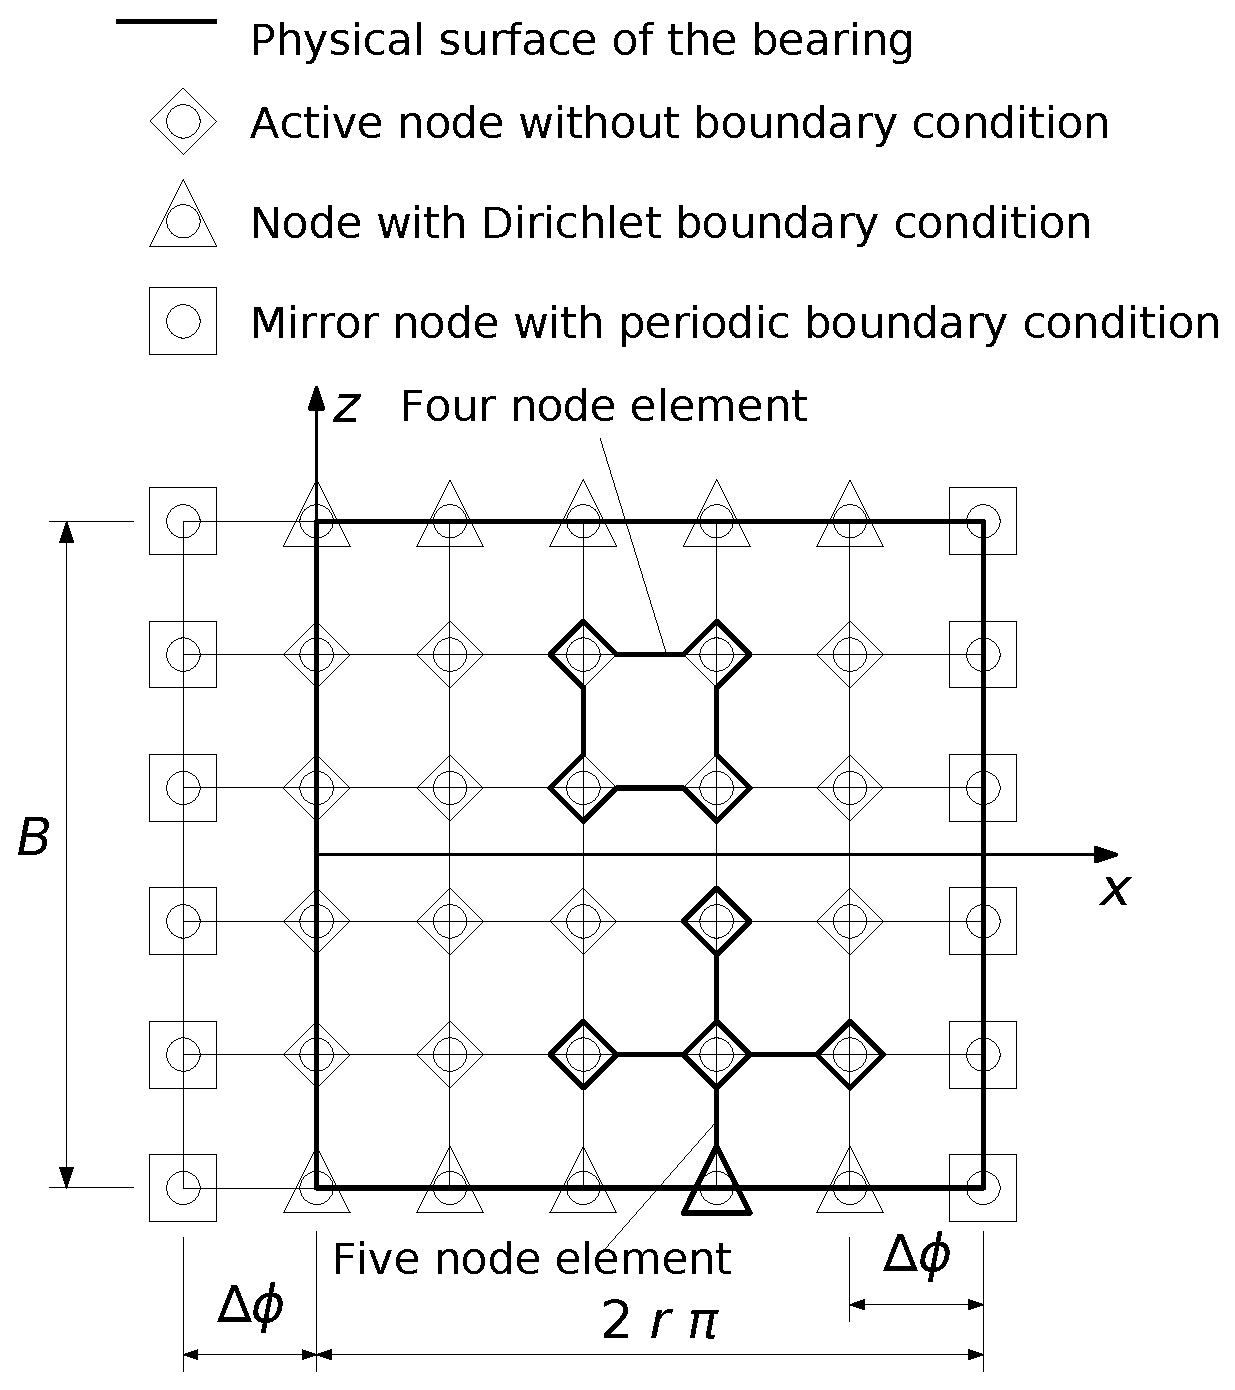
\includegraphics[width=0.5\linewidth]{fig_h150en}
\caption{orthogonal finite difference mesh of a cylindrical journal bearing}
\label{fig:h150}
\end{figure}

\subsection{The compressible Reynolds differential equation}
\begin{IEEEeqnarray}{rCl}
\left.\frac{\partial p}{\partial x} \right\vert_{\textit{wc}} & \approx & \frac{\left. p \right\vert_{\textit{center}} - \left. p \right\vert_{\textit{west}}}{\left. x \right\vert_{\textit{center}} -\left. x \right\vert_{\textit{west}}} \\
\left. h \right\vert_{\textit{wc}}&\approx&\frac{1}{2}\,\left(\left. h\right\vert_{\textit{west}} + \left. h \right\vert_{\textit{center}}\right) \\
\left. \Delta U_{1x} \right\vert_{\textit{wc}} &\approx& \frac{1}{2}\,\left(\left. \Delta U_{1x} \right\vert_{\textit{west}} + \left. \Delta U_{1x} \right\vert_{\textit{center}}\right)\\
\left. \Delta U_{2x} \right\vert_{\textit{wc}} &\approx& \frac{1}{2}\,\left(\left. \Delta U_{2x} \right\vert_{\textit{west}} + \left. \Delta U_{2x} \right\vert_{\textit{center}}\right)\\
\left. q_x \right\vert_{\textit{wc}} & \approx & \frac{\left. \Delta U_{1x} \right\vert_{\textit{wc}} + \left. \Delta U_{2x} \right\vert_{\textit{wc}}}{2} \, \left. h \right\vert_{\textit{wc}} -\frac{\left. h^3 \right\vert_{\textit{wc}}}{12\,\eta} \, \left. \frac{\partial p}{\partial x}\right\vert_{\textit{wc}} \\
\left. \rho \right\vert_{\textit{wc}} & \approx & \left\{
\begin{array}{ll}
    \left.\rho\right\vert_{\textit{west}} & \text{wenn} \qquad q_x\vert_{\textit{wc}} \geq 0 \\
    \left.\rho\right\vert_{\textit{center}} & \text{wenn} \qquad q_x\vert_{\textit{wc}} < 0
\end{array} \right. \\
\left. \eta \right\vert_{\textit{wc}} & \approx & \frac{1}{2} \, \left(\left.\eta\right\vert_{\textit{west}} + \left. \eta \right\vert_{\textit{center}} \right) \\
\dot{m}_x\vert_{\textit{wc}} & \approx & \left. \rho \right\vert_{\textit{wc}} \, \left. q_x \right\vert_{\textit{wc}} \\
\left. \frac{\partial \dot{m}_x}{\partial x} \right\vert_{\textit{center}} & \approx & \frac{\dot{m}_x\vert_{\textit{ce}} - \dot{m}_x\vert_{\textit{wc}}}{x\vert_{\textit{ce}} - x\vert_{\textit{wc}}} \\
\left. \frac{\partial \dot{m}_z}{\partial z} \right\vert_{\textit{center}} & \approx & \frac{\dot{m}_z\vert_{\textit{cn}} - \dot{m}_z\vert_{\textit{sc}}}{z\vert_{\textit{cn}} - z\vert_{\textit{sc}}} \\
\left. \frac{\partial}{\partial t}\,\left(\rho \, h\right)\right\vert_{\textit{center}} & \approx & \frac{\partial}{\partial t}\,\left(\left. \rho \right\vert_{\textit{center}} \, \left. h \right\vert_{\textit{center}}\right)
\end{IEEEeqnarray}

\subsubsection{The Courant Friedrichs Lewy condition}
Since the compressible Reynolds equation is of parabolic type, it is necessary to consider the CFL condition. This is for the two-dimensional case:
\begin{IEEEeqnarray}{rCl}
\Delta t & \leq & \frac{C_{max}}{\frac{q_x}{h\,\Delta x} + \frac{q_z}{h\,\Delta z}}
\end{IEEEeqnarray}
The CFL condition is checked in the multibody system in each iteration after the calculation of the residual and the time step size is reduced accordingly if necessary. For explicit methods, $C_{max}=1$ usually applies. However, since the solution method used is implicit, it is also possible that $C_{max} \geq 1$ is specified. However, values of $C_{max}$ that are too high can lead to divergence of the non-linear solver.

\section{Hydraulic boundary conditions}
\subsection{Dirichlet boundary condition}
Dirichlet boundary conditions can be specified either for the hydraulic pressure $p$ or for the density $\rho$ or for the radial gap height $h_0$ filled with oil.

\subsubsection{Partially flooded bearing edges}
In this case, it is assumed that the component surface on the opposite side of the mesh is wetted with an oil film with a layer thickness of $h_0$ at the bearing edges. See figure~\ref{fig:h350}.
\begin{figure}[htb]
\centering
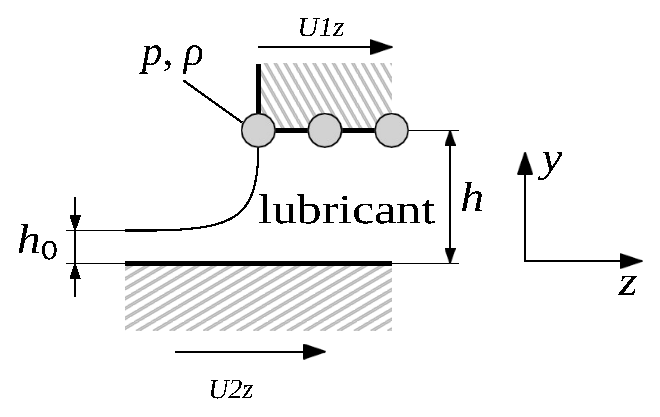
\includegraphics[width=0.5\linewidth]{fig_h350}
\caption{assumptions for partially flooded bearing edges}
\label{fig:h350}
\end{figure}
This assumption was made based on the commercial software AVL-Excite. In the case of the lubricating film of the piston, where the mesh is always on the piston, an oil film with a constant layer thickness $h_0$ on the cylinder liner is assumed because only in this case is oil transport through the bearing edges possible due to the axial movement of the piston. The fluid density at the bearing edges is determined as follows
\begin{IEEEeqnarray}{rCl}
\Phi & = & \frac{h_0}{h} \\
\rho & = & \left\{
\begin{array}{ll}
\rho_c \, \Phi & \text{when} \qquad \Phi \leq 1 \cr
\rho_c & \text{if} \qquad \Phi > 1
\end{array}
\right.
\end{IEEEeqnarray}
However, since Reynolds' differential equation only knows one independent variable, it is not possible to specify density and pressure at the bearing edges at the same time. In order to be able to specify pressure and density independently of each other, it would be necessary to switch to a multiphase flow which also takes into account the proportion of dissolved gas. However, such an approach was not pursued in this work.

\subsubsection{Coupling of boundary conditions with other variables}
When specifying a Dirichlet boundary condition, it is possible to specify not only constants but also any functions as boundary conditions. For example the pressure can be specified as a boundary condition for the lubricating film at the edges of a bearing, or within lubrication grooves, by means of a ``DriveCaller''.

\subsubsection{Geometric locations for the application of boundary conditions}
A Dirichlet boundary condition is always required at the bearing edges of the cylindrical plain bearing. In addition, lubrication grooves with a circular or rectangular cross-section can be defined and Dirichlet boundary conditions can be specified there. For reasons of accuracy, the mesh must be located at the same side as the lubrication grooves.

\subsection{Periodic boundary conditions}
Since the surface of the cylindrical plain bearing is unwound onto a plane, it is necessary that the radial bearing edges are coupled with each other. For this purpose, so-called mirror nodes were introduced which have their own nodal coordinates but obtain their value and equation number from their corresponding nodes at the opposite side of the mesh.

\subsection{Coupling a plain bearing with a hydraulic network}
In the multi-body system \href{http://www.mbdyn.org}{MBDyn} used, it is also possible to set up hydraulic networks consisting of pipelines, valves, throttle points, tanks and hydraulic actuators. For this reason, it was obvious to provide a coupling between individual plain bearings with a hydraulic network. In this way, for example, the two journal bearings may be connected to each other via a pipeline. The quantity of oil supplied via the oil pump can be specified as a function of the revolution speed, for example.

\subsubsection{Coupling at the bearing edges}
When coupling the mass flow through bearing edges with the hydraulic network, the following conditions apply for the bearing edge at $z=\frac{B}{2}$:
\begin{IEEEeqnarray}{rCl}
\left.p\right\vert_{z=\frac{B}{2}} & = & p_{hyd} \\
\dot{m}_{hyd} & = & -\int_{x=0}^{2\pi\,r} \left[\rho \, \left.\left(\frac{\Delta U_{1z} + \Delta
U_{2z}}{2} \, h - \frac{h^3}{12 \, \eta} \, \frac{\partial p}{\partial
z}\right)\right]\right\vert_{z=\frac{B}{2}} \, dx
\label{h:710}
\end{IEEEeqnarray}
\begin{description}
\item[$p_{hyd}$] Pressure of the node from the hydraulic network to which the bearing edge is coupled
\item[$\dot{m}_{hyd}$] Mass flow which emerges from the hydraulic network
\end{description}

The negative sign in equation~\ref{h:710} results from the convention for defining the residual for the nodes in the hydraulic network. Equation~\ref{h:710} applies if the network is located on the bearing journal. Otherwise, it must be integrated over $\int_{x=0}^{2\,\pi\,R}$.
\paragraph{Consideration of the flow direction for $z=-\frac{B}{2}$}
Coupling with the hydraulic network is achieved using four nodal coupling elements at the bearing edges. To couple the mass flow in the negative $z$ direction, the node coordinates are swapped in the $x$ direction so that $dx$ becomes negative.

\subsubsection{Coupling with a radial lubrication groove}
When coupling with a radial lubrication groove, the continuity equation is extended by an additional source term.
\begin{IEEEeqnarray}{rCl}
\left. p \right\vert_{A_{hyd}} & = & p_{hyd} \\
\dot{m}_{hyd} & = & \oint_{A_{hyd}} \left\{\frac{\partial \left(\rho \, h\right)}{\partial t} +
\frac{\partial}{\partial x}\left[\rho \, \left(\frac{\Delta U_{1x} + \Delta U_{2x}}{2} \, h - \frac{h^3}{12 \, \eta}
\, \frac{\partial p}{\partial x}\right)\right]\right. \nonumber \\
& & + \left.\frac{\partial}{\partial z}\left[\rho\,\left(\frac{\Delta U_{1z} + \Delta U_{2z}}{2}
\, h - \frac{h^3}{12 \, \eta} \, \frac{p}{z}\right)\right]\right\} \, dA_{hyd}
\end{IEEEeqnarray}
\begin{description}
\item[$A_{hyd}$] Area of the radial lubrication groove on the bearing surface
\end{description}
Pressure losses due to flow restrictions when entering the lubricating oil bore must be explicitly modeled in the hydraulic network by means of a throttling point. Coupling with a radial lubrication groove is only possible if this is located on the side of the mesh.

\section{Kinematic boundary conditions}
\label{sec:h100}
The kinematic variables $h$, $\frac{\partial h}{\partial t}=\dot{h}$, $\Delta \boldsymbol{U}_1$ and $\Delta \boldsymbol{U}_2$ required in equation~\ref{eq:h350} are derived in this section. Two possibilities have been implemented in this work so far:
\begin{itemize}
  \item The mesh moves with the bearing journal
  \item The mesh moves with the bearing shell
\end{itemize}
In the case of a piston-cylinder bearing, the first option must be selected so that the kinematic boundary conditions and the reaction forces correspond to reality. Both options can be used for radial plain bearings. The mesh should preferably be located on the side where the pockets or lubrication grooves are located in order to improve accuracy. However, it is also possible to specify pockets on the side opposite the mesh.

\subsection{The cylindrical plain bearing in which the mesh moves with the bearing journal}
\label{sec:h200}
The kinematic relationships in Equation~\ref{eq:h_1000} are shown in Figure~\ref{fig:h400}. It is assumed that the radial gap height vector $\boldsymbol{v}_h$ is normal to the surface of the bearing shell. Other assumptions would lead to a quadratic equation with multiple solutions. However, with the bearing clearances of $\Psi \approx 10^{-3}$ that are usual for radial plain bearings, the approximation used should be more than sufficiently accurate. For piston-cylinder bearings, the relative bearing clearance is even smaller than that.

\begin{figure}[htb]
\centering
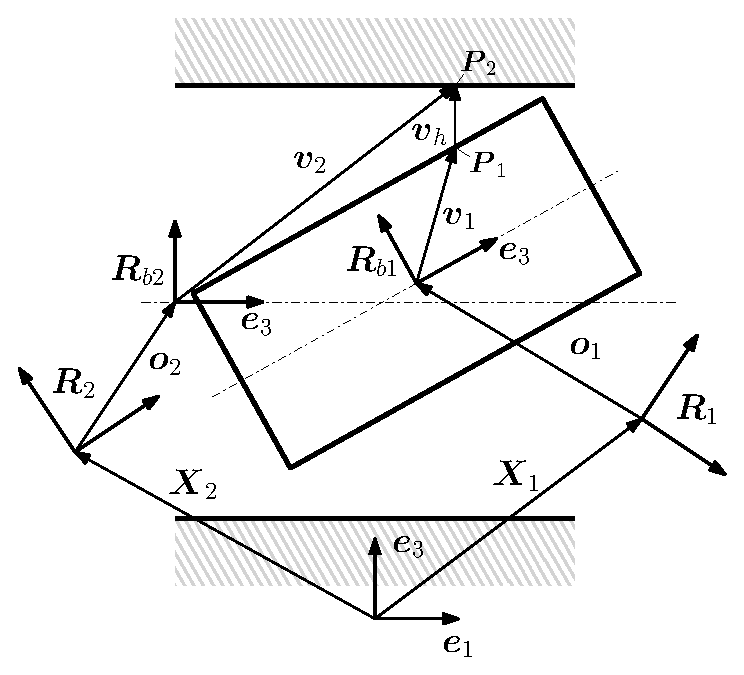
\includegraphics[width=0.5\linewidth]{fig_h400}
\caption{Kinematics of the rigid cylindrical plain bearing with mesh on the bearing journal}
\label{fig:h400}
\end{figure}

\subsubsection{The determination of the radial gap height}
\begin{IEEEeqnarray}{rCl}
\label{eq:h_1000}
\boldsymbol{X}_1 + \boldsymbol{R}_1 \, \left(\boldsymbol{o}_1 + \boldsymbol{R}_{b1} \,
\boldsymbol{v}_1\right) + \boldsymbol{R}_2 \, \boldsymbol{R}_{b2} \, \boldsymbol{v}_h & = &
\boldsymbol{X}_2 + \boldsymbol{R}_2 \, \left(\boldsymbol{o}_2 + \boldsymbol{R}_{b2} \,
\boldsymbol{v}_2\right)
\end{IEEEeqnarray}

\begin{description}
\item[$\boldsymbol{X}_1$] Position of the node of the bearing journal
\item[$\boldsymbol{R}_1$] Orientation of the node of the bearing journal
\item[$\boldsymbol{\omega}_1$] Angular velocity of the node of the bearing journal
\item[$\boldsymbol{o}_1$] Distance between the center of the bearing journal and the structural node of the bearing journal
\item[$\boldsymbol{R}_{b1}$] Orientation of the bearing journal relative to the node of the bearing journal
\item[$\boldsymbol{v}_1$] Distance from the center of the bearing journal to the point at the surface of the journal at which the radial gap height is measured, in the coordinate system of the journal
\item[$\boldsymbol{X}_2$] Position of the node of the bearing shell
\item[$\boldsymbol{R}_2$] Orientation of the node of the bearing shell
\item[$\boldsymbol{\omega}_2$] Angular velocity of the structural node of the bearing shell
\item[$\boldsymbol{o}_2$] Distance between the center of the bearing shell and the node of the bearing shell
\item[$\boldsymbol{R}_{b2}$] Orientation of the bearing shell relative to the structural node of the bearing shell
\item[$\boldsymbol{v}_2$] Distance from the center of the bearing shell to the point on the surface of the bearing shell at which the radial gap height is measured, in the coordinate system of the bearing shell
\item[$\boldsymbol{v}_h$] Vector of the radial gap height
\item[$h_{rb}$] Radial gap height, not considering elastic deformations of the bearing surfaces
\item[$h$] Actual radial gap height
\item[$w_{tot}$] Total radial component of the elastic deformation of the surfaces of bearing shell and bearing journal
\end{description}

For a certain node on the bearing journal, the vector $\boldsymbol{v}_1$ is known a priori according to equation~\ref{eq:h_1100}. The unknown variables in equation~\ref{eq:h_1200} and equation~\ref{eq:h_1300} are $\varphi_2$ and $h_{rb}$. These must be determined so that equation~\ref{eq:h_1000} is fulfilled.
\begin{IEEEeqnarray}{rCl}
\label{eq:h_1100}
\boldsymbol{v}_1 & = &
\begin{pmatrix}
\left(r + \Delta y_1\right) \, \cos\varphi_1 \cr
\left(r + \Delta y_1\right) \, \sin\varphi_1 \cr
z_1
\end{pmatrix} \\
\label{eq:h_1200}
\boldsymbol{v}_2 & = &
\begin{pmatrix}
\left(R + \Delta y_2\right) \, \cos\varphi_2 \cr
\left(R + \Delta y_2\right) \, \sin\varphi_2 \cr
z_2
\end{pmatrix} \\
\label{eq:h_1300}
\boldsymbol{v}_h & = &
\begin{pmatrix}
h_{rb} \, \cos\varphi_2 \\
h_{rb} \, \sin\varphi_2 \\
0
\end{pmatrix}
\end{IEEEeqnarray}
\begin{description}
\item[$\begin{pmatrix} \varphi_1 & z_1 \end{pmatrix}$] Position of the hydrodynamic node on the bearing journal in cylindrical coordinates
\item[$\Delta y_1$] Deviation of the journal surface with respect to the ideal cylindrical shape within specified areas (e.g. barrel shape, cone shape, ellipse shape, grooves, $\hdots$).
\item[$\begin{pmatrix} \varphi_2 & z_2 \end{pmatrix}$] Position of the point on the surface of the bearing shell which is opposite the hydrodynamic node on the bearing journal
\item[$\Delta y_2$] Deviation of the bearing shell surface with respect to the ideal cylindrical surface within specified areas (e.g. barrel shape, cone shape, ellipse shape, grooves, $\hdots$).
\end{description}

Due to the assumption that the vector $\boldsymbol{v}_h$ is normal to the surface of the bearing shell, the resolution of equation~\ref{eq:h_1000} to $\varphi_2$ and $h_{rb}$ is simple:
\begin{IEEEeqnarray}{rCl}
\boldsymbol{v}_2 -
\boldsymbol{v}_h & = & \underbrace{\boldsymbol{R}_{b2}^T \, \left\{\boldsymbol{R}_2^T \,
\left[\boldsymbol{X}_1 + \boldsymbol{R}_1 \, \left(\boldsymbol{o}_1 + \boldsymbol{R}_{b1} \, \boldsymbol{v}_1\right)
- \boldsymbol{X}_2\right]-\boldsymbol{o}_2\right\}}_{\boldsymbol{b}}
\end{IEEEeqnarray}
\begin{IEEEeqnarray}{rCl}
\begin{pmatrix}
\left[\left(R + \Delta y_2\right) - h_{rb}\right] \, \cos\varphi_2 \cr
\left[\left(R + \Delta y_2\right) - h_{rb}\right] \, \sin\varphi_2 \cr
z_2
\end{pmatrix} & = &
\begin{pmatrix}
b_1 \cr
b_2 \cr
b_3 \cr
\end{pmatrix} \\
\sin\varphi_2 & = & \frac{b_2}{\sqrt{b_1^2 + b_2^2}} \\
\cos\varphi_2 & = & \frac{b_1}{\sqrt{b_1^2 + b_2^2}} \\
\tan\varphi_2 & = & \frac{b_2}{b_1} \\
h_{rb} & = & R + \Delta y_2 - \sqrt{b_1^2 + b_2^2} \\
h & = & h_{rb} + w_{tot}
\end{IEEEeqnarray}

In addition, the derivatives of the radial gap height with respect to time are required for the Reynolds differential equation:
\begin{IEEEeqnarray}{rCl}
\dot{h}_{rb} & = & \Delta\dot{y}_2 - \frac{b_1 \, \dot{b}_1 + b_2 \, \dot{b}_2}{\sqrt{b_1^2 + b_2^2}}
\\
\dot{h} & = & \dot{h}_{rb} + \dot{w}_{tot} \\
\dot{\boldsymbol{b}} & = & \boldsymbol{R}_{b2}^T \, \boldsymbol{R}_2^T \,
\left\{\dot{\boldsymbol{X}}_1 + \left\langle \boldsymbol{\omega}_1 \right\rangle \,
\boldsymbol{R}_1 \, \left(\boldsymbol{o}_1 + \boldsymbol{R}_{b1} \, \boldsymbol{v}_1 \right)
- \dot{\boldsymbol{X}}_2 \right.\nonumber \\
& & \left.- \left\langle \boldsymbol{\omega}_2 \right\rangle \left[
\boldsymbol{X}_1 + \boldsymbol{R}_1 \, \left(\boldsymbol{o}_1 + \boldsymbol{R}_{b1} \,
\boldsymbol{v}_1 \right) - \boldsymbol{X}_2 \right]\right\}
\\
\Delta\dot{y}_2 & = & \frac{\partial \Delta y_2}{\partial x_2} \, \dot{x}_2 + \frac{\partial
\Delta y_2}{\partial z_2} \, \dot{z}_2 \\
\dot{x}_2 & = & R \, \dot{\varphi}_2 \\
\dot{\varphi}_2 & = & \frac{b_1 \, \dot{b}_2 - \dot{b}_1 \, b_2}{b_1^2 + b_2^2} \\
\dot{z}_2 & = & \dot{b}_3
\end{IEEEeqnarray}

For this purpose, the derivatives of $\Delta y_2$ must be specified.

\subsubsection{Deviations from the cylindrical bearing geometry}
Various types of so-called pockets were implemented in this work. A pocket is a deviation from the cylindrical bearing geometry within a given boundary. Rectangular and circular boundaries are currently implemented. If a node is located within this boundary, then $\Delta y_1$ or $\Delta y_2$ correspond to the height of the respective pocket. In the case of a circular boundary, this is of course only a very rough approximation. In the case of a rectangular boundary, it is still possible to align the grid lines accordingly when generating the mesh.
\paragraph{Pocket with constant height $\Delta y$}
In this case, the specified height $\Delta y$ applies to the entire area within the boundary. This means that $\frac{\partial \Delta y}{\partial x}=0$ and $\frac{\partial \Delta
y}{\partial z}=0$.

\paragraph{Pocket with linear interpolation of $\Delta y$}
With linear interpolation, the height $\Delta y$ can be specified at four vertices of a rectangle. See figure~\ref{fig:h500}. The rectangle is only used for interpolation or extrapolation. The boundary of the pocket, on the other hand, can also be a circle, for example.

\begin{figure}[htb]
\centering
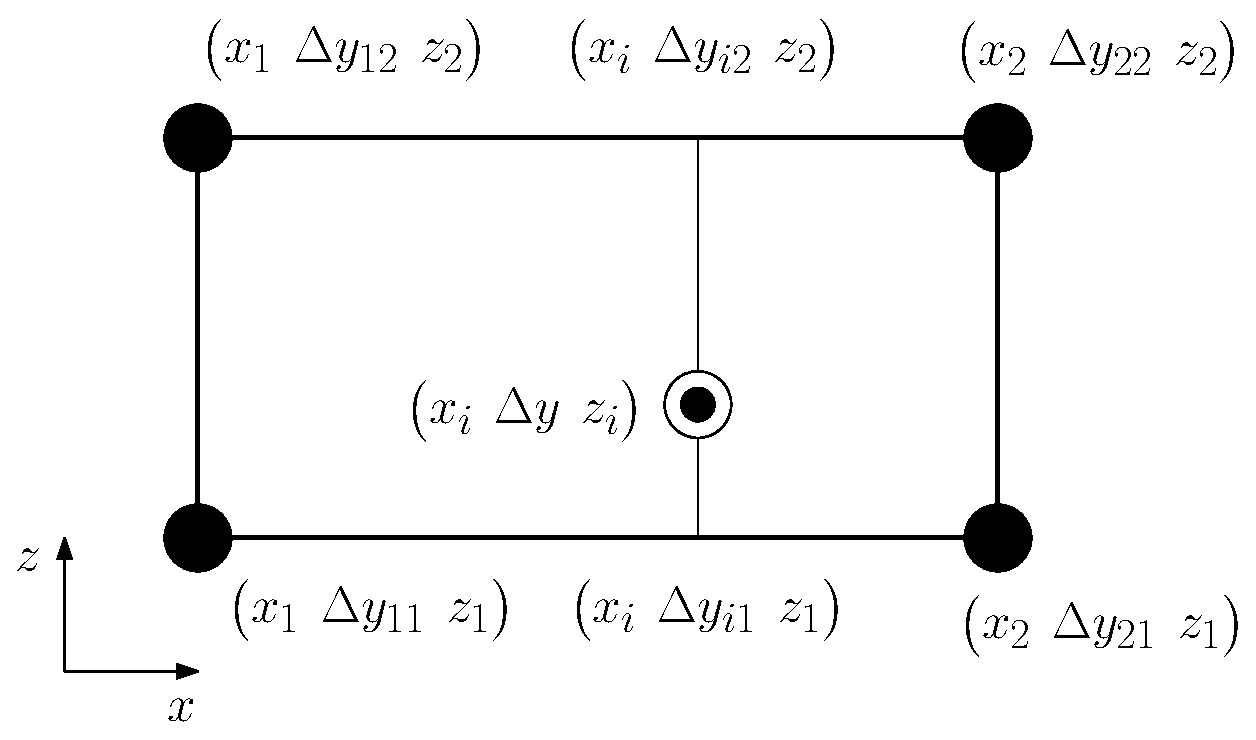
\includegraphics[width=0.5\linewidth]{fig_h500}
\caption{Interpolation of $\Delta y$ for a rectangular pocket}
\label{fig:h500}
\end{figure}

\begin{IEEEeqnarray}{rCl}
\Delta y_{i1} & = & \left(\Delta y_{21} - \Delta y_{11}\right) \, \frac{x_i - x_1}{x_2 - x_1} +
\Delta y_{11} \\
\Delta y_{i2} & = & \left(\Delta y_{22} - \Delta y_{12}\right) \, \frac{x_i - x_1}{x_2 - x_1} +
\Delta y_{12} \\
\Delta y & = & \left(\Delta y_{i2} - \Delta y_{i1}\right) \, \frac{z_i - z_1}{z_2 - z_1} +
\Delta y_{i1} \\
\frac{\partial \Delta y}{\partial x} & = & \frac{z_i - z_1}{z_2 - z_1} \,
\left(\frac{\partial \Delta y_{i2}}{\partial x} - \frac{\partial \Delta y_{i1}}{\partial x}\right) +
\frac{\partial \Delta y_{i1}}{\partial x} \\
\frac{\partial \Delta y_{i1}}{\partial x} & = & \frac{\Delta y_{21} - \Delta y_{11}}{x_2 - x_1} \\
\frac{\partial \Delta y_{i2}}{\partial x} & = & \frac{\Delta y_{22} - \Delta y_{12}}{x_2 - x_1} \\
\frac{\partial \Delta y}{\partial z} & = & \frac{\Delta y_{i2} - \Delta y_{i1}}{z_2 - z_1}
\end{IEEEeqnarray}

\subsubsection{boundary conditions for the velocities}
The velocities $\Delta\boldsymbol{U}_1$ and $\Delta\boldsymbol{U}_2$ must still be specified for the Reynolds differential equation. For this purpose, the velocity of the points $\boldsymbol{P}_1$ and $\boldsymbol{P}_2$ which are located on the surface of the bearing journal and bearing shell are first determined as shown in figure~\ref{fig:h400}.
\begin{IEEEeqnarray}{rCl}
\boldsymbol{P}_1 & = & \boldsymbol{X}_1 + \boldsymbol{R}_1 \, \left(\boldsymbol{o}_1 +
\boldsymbol{R}_{b1} \, \boldsymbol{v}_1\right) \\
\boldsymbol{P}_2 & = & \boldsymbol{X}_2 + \boldsymbol{R}_2 \, \left(\boldsymbol{o}_2 +
\boldsymbol{R}_{b2} \, \boldsymbol{v}_2 \right)
\end{IEEEeqnarray}

For the absolute velocities of the points $\boldsymbol{P}_1$ and $\boldsymbol{P}_2$ we get
\begin{IEEEeqnarray}{rCl}
\dot{\boldsymbol{P}}_1 & = & \dot{\boldsymbol{X}}_1 +
\left\langle \boldsymbol{\omega}_1 \right\rangle \, \boldsymbol{R}_1 \,
\left(\boldsymbol{o}_1 + \boldsymbol{R}_{b1} \, \boldsymbol{v}_1 \right) \\
\dot{\boldsymbol{P}}_2 & = & \dot{\boldsymbol{X}}_2 + \left\langle \boldsymbol{\omega}_2
\right\rangle \, \boldsymbol{R}_2 \, \left(\boldsymbol{o}_2 + \boldsymbol{R}_{b2} \,
\boldsymbol{v}_2 \right)
\end{IEEEeqnarray}

Finally, the difference between the absolute velocities of the component surface and the control volume is transformed into the tangential coordinate system $\boldsymbol{R}_{t1}$. The orientation of the tangential coordinate system is shown in Figure~\ref{fig:h_700}. Since the mesh moves with the bearing journal according to the assumptions in this section, the velocity difference $\Delta\boldsymbol{U}_1$ at the bearing journal is zero.

\begin{IEEEeqnarray}{rCl}
\Delta\boldsymbol{U}_1 & = & \boldsymbol{0} \\
\Delta \boldsymbol{U}_2 & = & \boldsymbol{R}_{t1}^T \, \boldsymbol{R}_{b1}^T \, \boldsymbol{R}_1^T
\, \left(\dot{\boldsymbol{P}}_2 - \dot{\boldsymbol{P}}_1\right) \\
\boldsymbol{R}_{t1} & = & \begin{pmatrix}
-\sin\varphi_1 & -\cos\varphi_1 & 0 \cr
\cos\varphi_1 & -\sin\varphi_1 & 0 \cr
0 & 0 & 1
\end{pmatrix}
\end{IEEEeqnarray}

\begin{figure}[htb]
\centering
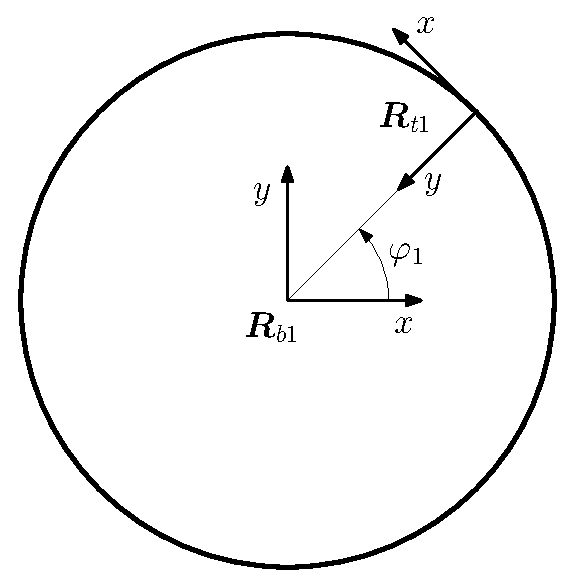
\includegraphics[width=0.3\linewidth]{fig_h700}
\caption{Orientation of the tangential coordinate system}
\label{fig:h_700}
\end{figure}

\subsection{The cylindrical plain bearing in which the mesh moves with the bearing shell}
It is assumed that the radial gap height $\boldsymbol{v}_h$ is measured normal to the surface of the bearing journal. See figure~\ref{fig:h600}. Apart from this, the kinematic relationships are the same as in section~\ref{sec:h200}.
\begin{figure}[htb]
\centering
\includegraphics[width=0.5\linewidth]{fig_h600}
\caption{Kinematics of the cylindrical plain bearing with mesh on the bearing shell}
\label{fig:h600}
\end{figure}

\subsubsection{The determination of the radial gap height}
\begin{IEEEeqnarray}{rCl}
\boldsymbol{v}_h & = &
\begin{pmatrix}
h_{rb} \, \cos\varphi_1 \cr
h_{rb} \,  \sin\varphi_1 \cr
0 \end{pmatrix} \\
\boldsymbol{v}_1 + \boldsymbol{v}_{h} & = & \boldsymbol{b} \nonumber \\
& = & \boldsymbol{R}_{b1}^T
\, \left\{ \boldsymbol{R}_1^T \, \left[\boldsymbol{X}_2 + \boldsymbol{R}_2 \, \left(\boldsymbol{o}_2 + \boldsymbol{R}_{b2} \,
\boldsymbol{v}_2 \right) - \boldsymbol{X}_1\right] - \boldsymbol{o}_1 \right\} \\
\dot{\boldsymbol{b}} & = & \boldsymbol{R}_{b1}^T \, \boldsymbol{R}_1^T \, \left\{\dot{X}_2 +
\left\langle \boldsymbol{\omega}_2 \right\rangle \, \boldsymbol{R}_2 \,
\left(\boldsymbol{o}_2 + \boldsymbol{R}_{b2} \, \boldsymbol{v}_2\right) - \dot{\boldsymbol{X}}_1
\right. \nonumber \\
& & \left.- \left\langle\boldsymbol{\omega}_1\right\rangle \, \left[\boldsymbol{X}_2 +
\boldsymbol{R}_2 \, \left(\boldsymbol{o}_2 + \boldsymbol{R}_{b2} \, \boldsymbol{v}_2\right) -
\boldsymbol{X}_1\right]\right\} \\
\end{IEEEeqnarray}


\begin{IEEEeqnarray}{rCl}
\sin\varphi_1 & = & \frac{b_2}{\sqrt{b_1^2 + b_2^2}} \\
\cos\varphi_1 & = & \frac{b_1}{\sqrt{b_1^2 + b_2^2}} \\
\tan\varphi_1 & = & \frac{b_2}{b_1} \\
\dot{\varphi}_1 & = & \frac{b_1 \, \dot{b}_2 - \dot{b}_1 \, b_2}{b_1^2 + b_2^2} \\
h_{rb} & = & \sqrt{b_1^2 + b_2^2} - r - \Delta y_1 \\
\dot{h}_{rb} & = & \frac{b_1 \, \dot{b}_1 + b_2 \, \dot{b}_2}{\sqrt{b_1^2 + b_2^2}} - \Delta\dot{y}_1 \\
h & = & h_{rb} + w_{tot} \\
\dot{h} & = & \dot{h}_{rb} + \dot{w}_{tot} \\
\Delta\dot{y}_1 & = & \frac{\partial \Delta y_1}{\partial x_1} \, \dot{x}_1 + \frac{\partial\Delta y_1}{\partial z_1}\,\dot{z}_1 \\
\dot{x}_1 & = & r \, \dot{\varphi}_1 \\
\dot{z}_1 & = & \dot{b}_3
\end{IEEEeqnarray}

\subsubsection{Boundary conditions for the velocities}
In contrast to section~\ref{sec:h200}, the following applies to the velocities:
\begin{IEEEeqnarray}{rCl}
\Delta \boldsymbol{U}_1 & = & \boldsymbol{R}_{t2}^T \, \boldsymbol{R}_{b2}^T \, \boldsymbol{R}_2^T
\, \left(\dot{\boldsymbol{P}}_1 - \dot{\boldsymbol{P}}_2\right) \\
\Delta \boldsymbol{U}_2 & = & \boldsymbol{0}\\
\boldsymbol{R}_{t2} & = & \begin{pmatrix}
-\sin\varphi_2 & -\cos\varphi_2 & 0 \cr
\cos\varphi_2 & -\sin\varphi_2 & 0 \cr
0 & 0 & 1
\end{pmatrix}
\end{IEEEeqnarray}

\section{Solid body contact and dry friction}
\subsection{The contact model of Greenwood and Tripp}
In order to account for solid contact and dry friction between rough surfaces, the approach of Greenwood and Tripp was applied\cite{Greenwood-1970}. The equations for the Hertzian contact pressure between asperities of rough surfaces are \cite{Greenwood-1970}:
\begin{IEEEeqnarray}{rCl}
p_{asp} & = & \frac{16\,\sqrt{2}}{15} \, \pi \, \left(\eta_{asp} \, \beta_{asp} \sigma_{\delta}\right)^2
\, \acute{E} \, \sqrt{\frac{\sigma_{\delta}}{\beta_{asp}}} \,
F_{\frac{5}{2}}\left(\frac{h}{\sigma_{\delta}}\right) \\
\acute{E} & = & \left(\frac{1 - \nu_1^2}{E_1} + \frac{1 - \nu_2^2}{E_2}\right)^{-1} \\
F_{\frac{5}{2}}\left(H\right) & = & \left\{
\begin{array}{ll}
4.4086 \cdot 10^{-5} \, \left(4 -H\right)^{6.804} & \text{if} \qquad H \leq 4 \cr
0 & \text{if} \qquad H > 4
\end{array} \right. \\
H &=& \frac{h}{\sigma_{\delta}} \\
\sigma_{\delta} & = & \sqrt{M_0} \\
\eta_{asp} & = & \frac{1}{6 \, \pi \, \sqrt{3}} \, \frac{M_4}{M_2} \\
\beta_{asp} & = & \frac{3 \, \sqrt{\pi}}{8 \, \sqrt{M_4}}
\end{IEEEeqnarray}
\begin{description}
\item[$p_{asp}$] Pressure due to contact between the asperities of the rough surfaces
\item[$\eta_{asp}$] Asperity density
\item[$\beta_{asp}$] Radius of curvature of the asperity tip
\item[$\sigma_{\delta}$] Variance of the measured values of the roughness profile
\item[$M_0=\sigma_{\delta}^2$] combined zeroth spectral moment to describe the surface roughness
\item[$M_2=\dot{\sigma}_{\delta}^2$] combined second spectral moment to describe the surface roughness
\item[$M_4=\ddot{\sigma}_{\delta}^2$] combined fourth spectral moment to describe the surface roughness
\end{description}

According to \cite{Tomanik-2003}, those values can be determined from the analysis of measured roughness profiles of the component surfaces.

\subsection{The two-dimensional LuGre solid friction model} \label{sec:h500}
The standard model for the description of dry friction between solid bodies is Coulomb's law. However, the implementation of the transition between sliding friction and static friction for the general two-dimensional case is not trivial. The consideration of this transition is always important in a multi-body system, if the relative movement of a mechanism is going to stop due to friction. If sliding friction were always used in the calculation, an explicit integration scheme would result in endless oscillations around the static equilibrium point. For this reason, the two-dimensional LuGre model presented in \cite{LuGre2D} was selected, which is based on a linear differential equation and does not require any case distinctions. The LuGre friction model assumes that two bodies with rough surfaces touch each other at the tips of the asperities, also called bristles in the literature. With small relative movements, these bristles behave like springs. However, as soon as a certain maximum deformation is reached, the bristles begin to slide over each other. However, the transition between sticking and sliding is continuous in the LuGre model. The two-dimensional LuGre model from \cite{LuGre2D} reads:
\begin{IEEEeqnarray}{rCl}
\boldsymbol{\tau}_{asp} & = & \left(\boldsymbol{\sigma}_0 \, \boldsymbol{z} +
\boldsymbol{\sigma}_1
\,
\dot{\boldsymbol{z}}\right) \, p_{asp} \\
\dot{\boldsymbol{z}} & = & \Delta\boldsymbol{U} - \kappa \,
\boldsymbol{M}_{k}^{-2} \, \boldsymbol{\sigma}_0 \, \boldsymbol{z} \\
g & = & \frac{\left\Vert \boldsymbol{M}_k^2 \, \Delta\boldsymbol{U} \right\Vert}{\left\Vert
\boldsymbol{M}_k \, \Delta\boldsymbol{U}\right\Vert} + \left(\frac{\left\Vert \boldsymbol{M}_s^2 \, \Delta\boldsymbol{U} \right\Vert}{\left\Vert
\boldsymbol{M}_s \, \Delta\boldsymbol{U}\right\Vert} - \frac{\left\Vert \boldsymbol{M}_k^2 \, \Delta\boldsymbol{U} \right\Vert}{\left\Vert
\boldsymbol{M}_k \, \Delta\boldsymbol{U}\right\Vert}\right)\,\exp{\left[-\left(\frac{\left\Vert
\Delta\boldsymbol{U}\right\Vert}{v_s}\right)^\gamma\right]} \\
\kappa & = & \frac{\left\Vert \boldsymbol{M}_k^2 \, \Delta\boldsymbol{U}\right\Vert}{g} \\
\boldsymbol{M}_k & = & \begin{pmatrix}
\mu_{kx} & 0 \cr
0 & \mu_{kz}
\end{pmatrix} \\
\boldsymbol{M}_s & = & \begin{pmatrix}
\mu_{sx} & 0 \cr
0 & \mu_{sz}
\end{pmatrix} \\
\boldsymbol{\sigma}_0 & = & \begin{pmatrix}
\sigma_{0x} & 0 \cr
0 & \sigma_{0z}
\end{pmatrix} \\
\boldsymbol{\sigma}_1 & = & \begin{pmatrix}
\sigma_{1x} & 0 \cr
0 & \sigma_{1z}
\end{pmatrix} \\
\Delta\boldsymbol{U} & = & \begin{pmatrix}
\boldsymbol{e}_1^T \cr
\boldsymbol{e}_3^T
\end{pmatrix} \,
\left(\Delta\boldsymbol{U}_1 - \Delta\boldsymbol{U}_2\right)
\end{IEEEeqnarray}
\begin{description}
\item[$\boldsymbol{z} = \begin{pmatrix} z_1 \cr z_2 \end{pmatrix}$] Deformation of the bristles
\item[$\boldsymbol{\tau}_{asp} = \begin{pmatrix} \tau_{asp_{xy}} \cr
\tau_{asp_{yz}}\end{pmatrix}$] Shear stresses due to dry friction
\item[$\Delta\boldsymbol{U}$] Components of the velocity difference in $x$- and $z$~direction
\item[$\boldsymbol{\sigma}_0$] transient micro-sliding stiffness matrix
\item[$\boldsymbol{\sigma}_1$] transient micro-slip damping matrix
\item[$\boldsymbol{M}_k$] sliding friction matrix
\item[$\mu_{kx}$] coefficient of sliding friction in $x$~direction
\item[$\mu_{kz}$] Sliding friction coefficient in $z$~direction
\item[$\boldsymbol{M}_s$] static friction matrix
\item[$\mu_{sx}$] Coefficient of static friction in $x$~direction
\item[$\mu_{sz}$] Coefficient of static friction in $z$~direction
\item[$v_s$] Velocity which describes the transition between static friction and dynamic friction (Stribeck effect)
\item[$\gamma$] Coefficient that describes the transition between static friction and dynamic friction (Stribeck effect)
\end{description}

\subsubsection{The transition to Coulomb's law of friction}
For the stationary sliding process for isotropic surfaces without Stribeck effect, the LuGre model can be simplified as follows for illustrative purposes:
\begin{IEEEeqnarray}{rClrCl}
\dot{\boldsymbol{z}} & = & \boldsymbol{0}  \\
\boldsymbol{M}_k & = & \boldsymbol{M}_s \label{eq:h723} \\
\sigma_{0x} & = & \sigma_{0z} & = & \sigma_0 \label{eq:h724} \\
\mu_{kx} & = & \mu_{kz} & = & \mu_k \label{eq:h725}
\end{IEEEeqnarray}
With these simplifications we get
\begin{IEEEeqnarray}{rCl}
\boldsymbol{z} & = & \frac{\mu_k}{\sigma_0 \, \left\Vert \Delta\boldsymbol{U}\right\Vert_2} \,
\Delta\boldsymbol{U} \\
\boldsymbol{\tau}_{asp} & = & \boldsymbol{\sigma}_0 \, \boldsymbol{z} \, p_{asp} \nonumber \\
& = & \frac{\mu_k \, p_{asp}}{\left\Vert \Delta\boldsymbol{U} \right\Vert_2} \, \Delta\boldsymbol{U}
\label{eq:h750}
\end{IEEEeqnarray}
Equation~\ref{eq:h750} therefore corresponds exactly to the surface area of the cone in Coulomb's law of friction.

\subsubsection{The transition to static friction}
For the unsteady one-dimensional case, the simplifications of equation~\ref{eq:h723}-\ref{eq:h725}:
\begin{IEEEeqnarray}{rCl}
\dot{z}_x & = & \Delta U_x - \left\vert \Delta U_x \right\vert \, \frac{\sigma_{0x}}{\mu_k} \, z_x
\label{eq:h770}
\end{IEEEeqnarray}

At constant velocity $\Delta U_x$, the analytical solution of the differential equation~\ref{eq:h770} and the initial condition $\left.z_x\right\vert_{t=0}=0$:
\begin{IEEEeqnarray}{rCl}
z_x & = & \left[1 - \exp{\left(-\left\vert \Delta U_x \right\vert \,
\frac{\sigma_{0x}}{\mu_k} \, t\right)}\right] \, \frac{\mu_k}{\sigma_{0x}} \, \sign{\Delta U_x} \\
\tau_x & = & \left[\mu_k \, \sign{\Delta U_x} + \left(\Delta U_x \, \sigma_{1x} - \mu_k \,
\sign{\Delta U_x}\right) \, \exp{\left(-\left\vert \Delta U_x\right\vert
\, \frac{\sigma_{0x}}{\mu_k} \, t \right)}\right] \, p_{asp} \label{eq:h775}
\end{IEEEeqnarray}

Figure~\ref{fig:h900} shows the course of the shear stresses as a function of the deformation according to equation~\ref{eq:h775}. It can be seen from this that the product $\sigma_{0x} \, p_{asp}$ only indicates the gradient of the stress curve at the beginning of the movement (black straight line). After that, the movement changes into a creeping movement.
\begin{figure}[htb]
\centering
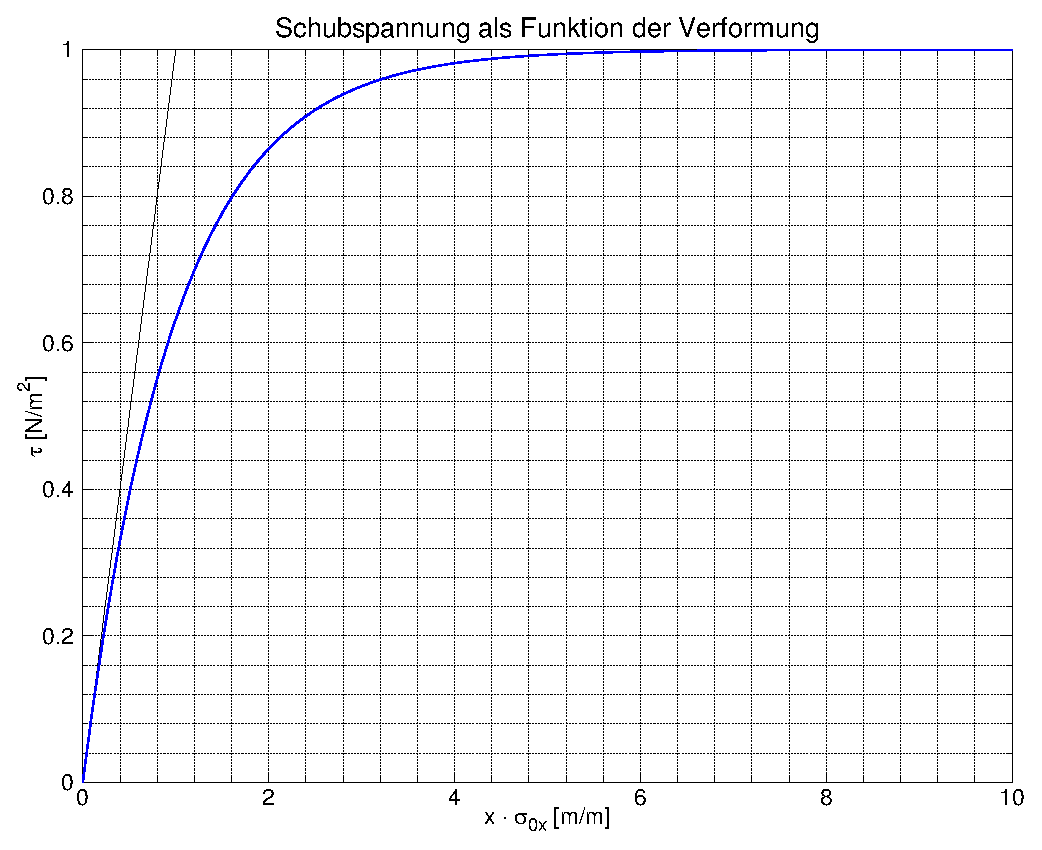
\includegraphics[width=0.5\linewidth]{fig_h900}
\caption{Shear stress distribution as a function of deformation in the one-dimensional LuGre model}
\label{fig:h900}
\end{figure}

\subsubsection{Numerical integration of the LuGre model}
In principle, the linear differential equation for the LuGre model could be solved together with the other equations of the multi-body system. However, this would triple the size of the Jacobian matrix, as the states $\boldsymbol{z}$ for the transition between static friction and dynamic friction would have to be stored for each node in addition to the hydrodynamic pressure $p$. However, since the differential equation of the LuGre model is linear and the static friction states of the individual nodes are independent, the LuGre model was numerically integrated separately from the other equations. The following integration scheme is used for this purpose:
\begin{IEEEeqnarray}{rCl}
\left.\boldsymbol{z}\right\vert_{t} & = & \left[\zeta \,
\left.\dot{\boldsymbol{z}}\right\vert_{t} + \left(1 - \zeta\right) \,
\left.\dot{\boldsymbol{z}}\right\vert_{t - 1}\right] \, \Delta t +
\left.\boldsymbol{z}\right\vert_{t - 1}
\end{IEEEeqnarray}

\begin{description}
\item[$\Delta t$] time step size
\item[$\zeta=0$] explicit Euler method (unstable)
\item[$\zeta=\frac{1}{2}$] trapezoidal rule (second order accurate)
\item[$\zeta=1$] implicit Euler method (first order accurate)
\end{description}

With these assumptions, the following equation for $\dot{\boldsymbol{z}}$ results:
\begin{IEEEeqnarray}{rCl}
\left.\boldsymbol{A}\right\vert_t & = & \left.\kappa\right\vert_t \, \boldsymbol{M}_k^{-2} \,
\boldsymbol{\sigma}_0
\\
\left.\dot{\boldsymbol{z}}\right\vert_{t} & = & \left(\boldsymbol{I} + \zeta \, \Delta t \,
\left.\boldsymbol{A}\right\vert_t\right)^{-1} \, \left\{ \left.\Delta\boldsymbol{U}\right\vert_{t} -
\left.\boldsymbol{A}\right\vert_t \, \left[\left(1 - \zeta\right) \,
\left.\dot{\boldsymbol{z}}\right\vert_{t-1} \, \Delta t +
\left.\boldsymbol{z}\right\vert_{t-1}\right]\right\}
\end{IEEEeqnarray}

\section{Reaction forces}
\subsection{Frictional forces due to fluid friction}
For a Newtonian fluid in laminar flow, the shear stresses $\tau_{xy}$ and $\tau_{yz}$ apply:
\begin{IEEEeqnarray}{rCl}
\tau_{xy} & = & \eta \, \left(\frac{\partial u_x}{\partial y} + \underbrace{\frac{\partial
u_y}{\partial x}}_{\approx 0}\right) \nonumber \\
\tau_{yz} & = & \eta \, \left(\underbrace{\frac{\partial u_y}{\partial z}}_{\approx 0} +
\frac{\partial u_z}{\partial y}\right) \label{eq:h800}
\end{IEEEeqnarray}
As in the derivation of the Reynolds differential equation, the derivatives of the velocity in the circumferential direction and axial direction are neglected compared to the derivative in the radial gap height direction. If equation~\ref{eq:h325} is differentiated according to $y$, the velocity gradients are obtained:
\begin{IEEEeqnarray}{rCl}
\frac{\partial u_x}{\partial y} & = & \frac{1}{\eta} \, \frac{\partial p}{\partial x} \,
\left(y - \frac{h}{2}\right) + \frac{\Delta U_{1x} - \Delta U_{2x}}{h} \nonumber \\
\frac{\partial u_z}{\partial y} & = & \frac{1}{\eta} \, \frac{\partial p}{\partial z} \,
\left(y - \frac{h}{2}\right) + \frac{\Delta U_{1z} - \Delta U_{2z}}{h} \label{eq:h900}
\end{IEEEeqnarray}
Substituting equation~\ref{eq:h900} into equation~\ref{eq:h800} gives the shear stresses at the surface of the components:
\begin{IEEEeqnarray}{rCl}
\left.\tau_{xy}\right\vert_{y=0} & = & - \frac{h}{2} \, \frac{\partial
p}{\partial x} + \eta \, \frac{\Delta U_{1x} - \Delta U_{2x}}{h} \\
\left.\tau_{xy}\right\vert_{y=h} & = & \frac{h}{2} \, \frac{\partial
p}{\partial x} + \eta \, \frac{\Delta U_{1x} - \Delta U_{2x}}{h} \\
\left.\tau_{yz}\right\vert_{y=0} & = & - \frac{h}{2} \, \frac{\partial p}{\partial z} + \eta \,
\frac{\delta U_{1z} - \Delta U_{2z}}{h} \\
\left.\tau_{yz}\right\vert_{y=h} & = & \frac{h}{2} \, \frac{\partial p}{\partial z} + \eta \,
\frac{\delta U_{1z} - \Delta U_{2z}}{h}
\end{IEEEeqnarray}

\subsection{The mesh moves with the bearing shell}
\label{sec:h350}
The reaction forces on the bearing journal and on the bearing shell result from the integration of the shear stresses and the pressure loads over the surface. The kinematic relationships are shown in Figure~\ref{fig:h800}.

\begin{figure}[htb]
\centering
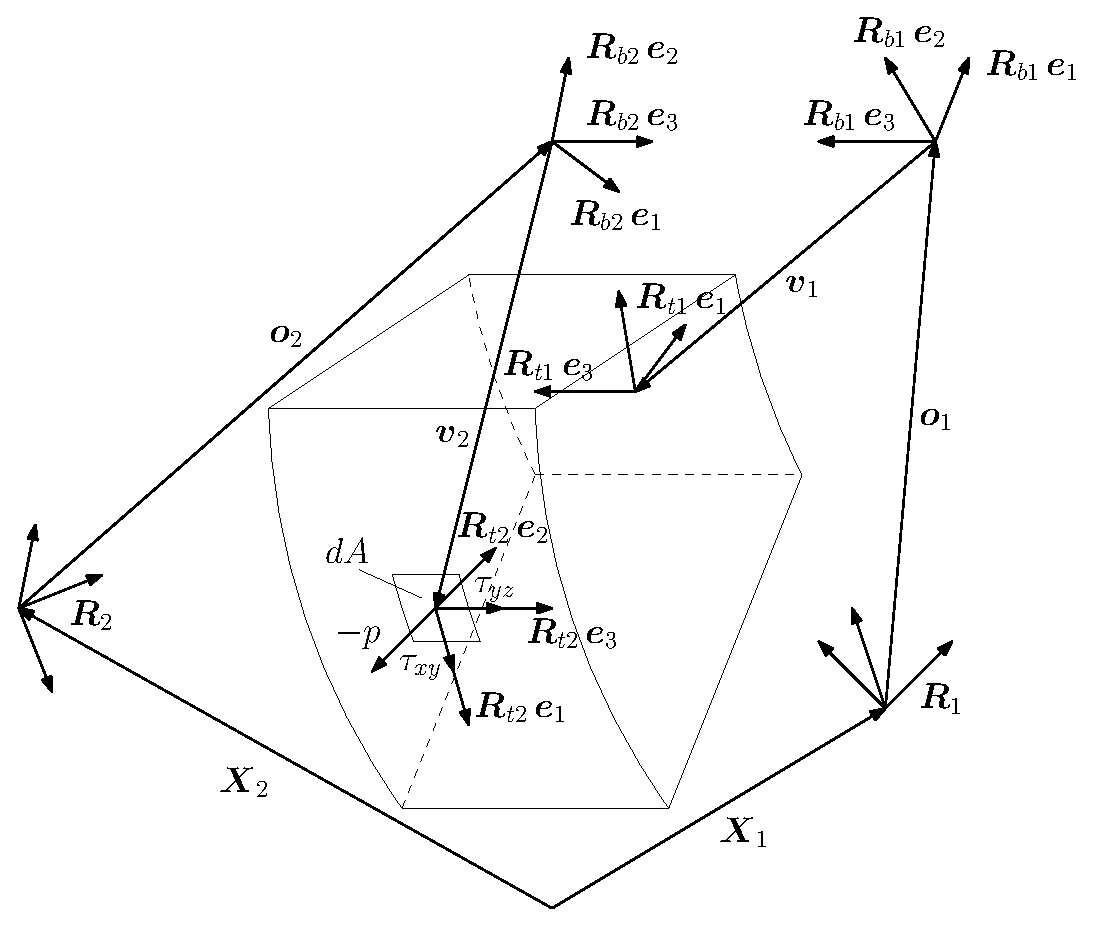
\includegraphics[width=0.5\linewidth]{fig_h800}
\caption{Reaction forces with a mesh on the bearing shell}
\label{fig:h800}
\end{figure}

\subsubsection{Forces on the bearing shell}
\label{sec:h300}
The integration of the reaction forces on the bearing shell is conveniently carried out in the coordinate system of the node of the bearing shell.
\begin{IEEEeqnarray}{rCl}
d\boldsymbol{F}_{2}^{\left(\boldsymbol{R}_2\right)} & = & \boldsymbol{R}_{b2} \, \boldsymbol{R}_{t2}
\,
\begin{pmatrix}
\left.\tau_{xy}\right\vert_{y=0} + \tau_{asp_{xy}} \cr
-\left(p + p_{asp}\right) \cr
\left.\tau_{yz}\right\vert_{y=0} + \tau_{asp_{yz}}
\end{pmatrix}
\, dA_2 \\
d\boldsymbol{M}_2^{\left(\boldsymbol{R}_2\right)} & = & \left\langle \boldsymbol{R}_{b2} \,
\boldsymbol{v}_2 \right\rangle \, d\boldsymbol{F}_2^{\left(\boldsymbol{R}_2\right)} \\
\boldsymbol{F}_2 & = & \boldsymbol{R}_2 \, \oint_{A_2}
d\boldsymbol{F}_2^{\left(\boldsymbol{R}_2\right)}
\\
\boldsymbol{M}_2 & = & \left\langle\boldsymbol{R}_2\,\boldsymbol{o}_2\right\rangle \,
\boldsymbol{F}_2 + \boldsymbol{R}_2 \, \oint_{A_2} d\boldsymbol{M}_2^{\left(\boldsymbol{R}_2\right)}
\end{IEEEeqnarray}

\subsubsection{Forces on the bearing journal}
\label{sec:h400}
Since the shear stresses due to fluid friction are different on the bearing journal at $y=h$ and on the bearing shell at $y=0$, the reaction forces on both sides must be integrated. For this purpose, the shear stresses must be transformed from the mesh to the opposite side. This transformation assumes that the pressure $p$ also acts perpendicular to the surface on the opposite side and that the shear stresses $\tau_{xy}$ and $\tau_{yz}$ lie in the tangential plane of the surface of the bearing journal. However, as the bearing journal can tilt relative to the bearing shell or the coordinate system $\boldsymbol{R}_{b1}$ can be oriented differently to the coordinate system $\boldsymbol{R}_{b2}$, the modified tangential coordinate system $\bar{\boldsymbol{R}}_{t1}$ is introduced. This is defined as follows:
\begin{IEEEeqnarray}{rCl}
\bar{\boldsymbol{R}}_{t1} \, \boldsymbol{e}_2 & = & \boldsymbol{R}_1 \, \boldsymbol{R}_{b1} \,
\boldsymbol{R}_{t1} \, \boldsymbol{e}_2 \\
\bar{\boldsymbol{R}}_{t1} \, \boldsymbol{e}_1 & = & \left\langle\bar{\boldsymbol{R}}_{t1} \,
\boldsymbol{e}_1 \right\rangle \, \boldsymbol{R}_2 \, \boldsymbol{R}_{b2} \, \boldsymbol{R}_{t2} \,
\boldsymbol{e}_3 \\
\bar{\boldsymbol{R}}_{t1} \, \boldsymbol{e}_3 & = & \left\langle \bar{\boldsymbol{R}}_{t1} \,
\boldsymbol{e}_1 \right\rangle \bar{\boldsymbol{R}}_{t1} \, \boldsymbol{e}_2
\end{IEEEeqnarray}
The axes of the coordinate system $\bar{\boldsymbol{R}}_{t1}$ must still be scaled accordingly.
\begin{IEEEeqnarray}{rCl}
\left\Vert \bar{\boldsymbol{R}}_{t1} \, \boldsymbol{e}_1 \right\Vert & \equiv & 1 \\
\left\Vert \bar{\boldsymbol{R}}_{t1} \, \boldsymbol{e}_2 \right\Vert & \equiv & 1 \\
\left\Vert \bar{\boldsymbol{R}}_{t1} \, \boldsymbol{e}_3 \right\Vert & \equiv & 1
\end{IEEEeqnarray}
If the bearing journal is tilted relative to the bearing shell, the axes $\bar{\boldsymbol{R}}_{t1}\,\boldsymbol{e}_1$ and $\boldsymbol{R}_{t2} \, \boldsymbol{e}_1$ are no longer parallel. However, as the relative bearing clearance $\Psi$ is very small with the usual bearing dimensions, this angle will be very small.

In contrast to section~\ref{sec:h300}, the integration of the reaction forces on the bearing journal takes place in the global coordinate system.

\begin{IEEEeqnarray}{rCl}
d\boldsymbol{F}_1 & = & \bar{\boldsymbol{R}}_{t1} \,
\begin{pmatrix}
\left.-\tau_{xy}\right\vert_{y=h} -\tau_{asp_{xy}} \cr
p + p_{asp} \cr
\left.-\tau_{yz}\right\vert_{y=h} - \tau_{asp_{yz}}
\end{pmatrix} \, dA_1 \\
d\boldsymbol{M}_1 & = & \left\langle \boldsymbol{R}_1 \, \boldsymbol{R}_{b1} \, \boldsymbol{v}_1
\right\rangle \, d\boldsymbol{F}_1 \\
\boldsymbol{F}_1 & = & \oint_{A_1} d\boldsymbol{F}_1 \\
\boldsymbol{M}_1 & = & \left\langle \boldsymbol{R}_1 \, \boldsymbol{o}_1 \right\rangle \,
\boldsymbol{F}_1 + \oint_{A_1} d\boldsymbol{M}_1
\end{IEEEeqnarray}

\subsection{The mesh moves with the bearing journal}
The procedure with the mesh on the bearing journal is the same as described in section~\ref{sec:h350}.
\subsubsection{Forces on the bearing journal}
The following applies to the forces on the bearing journal:
\begin{IEEEeqnarray}{rCl}
d\boldsymbol{F}_1^{\left(\boldsymbol{R}_1\right)} & = & \boldsymbol{R}_{b1} \, \boldsymbol{R}_{t1}
\,
\begin{pmatrix}
-\left.\tau_{xy}\right\vert_{y=h} - \tau_{asp_{xy}} \cr
p + p_{asp} \cr
-\left.\tau_{yz}\right\vert_{y=h} - \tau_{asp_{yz}}
\end{pmatrix}
\, dA_1 \\
d\boldsymbol{M}_1^{\left(\boldsymbol{R}_1\right)} & = & \left\langle \boldsymbol{R}_{b1} \,
\boldsymbol{v}_1 \right\rangle \, d\boldsymbol{F}_1^{\left(\boldsymbol{R}_1\right)} \\
\boldsymbol{F}_1 & = & \boldsymbol{R}_1 \, \oint_{A_1}
d\boldsymbol{F}_1^{\left(\boldsymbol{R}_1\right)}
\\
\boldsymbol{M}_1 & = & \left\langle \boldsymbol{R}_1 \, \boldsymbol{o}_1
\right\rangle \, \boldsymbol{F}_{1} + \boldsymbol{R}_1 \, \oint_{A_1}
d\boldsymbol{M}_1^{\left(\boldsymbol{R}_1\right)}
\end{IEEEeqnarray}

\subsubsection{Forces on the bearing shell}
The transformation of the forces from the bearing journal to the bearing shell is analogous to
Section~\ref{sec:h400}.
\begin{IEEEeqnarray}{rCl}
\bar{\boldsymbol{R}}_{t2} \, \boldsymbol{e}_2 & = & \boldsymbol{R}_2 \, \boldsymbol{R}_{b2} \,
\boldsymbol{R}_{t2} \, \boldsymbol{e}_2 \\
\bar{\boldsymbol{R}}_{t2} \, \boldsymbol{e}_1 & = & \left\langle \bar{\boldsymbol{R}}_{t2} \,
\boldsymbol{e}_2 \right\rangle \, \boldsymbol{R}_1 \, \boldsymbol{R}_{b1} \, \boldsymbol{R}_{t1} \,
\boldsymbol{e}_3 \\
\bar{\boldsymbol{R}}_{t2} \, \boldsymbol{e}_3 & = & \left\langle \bar{\boldsymbol{R}}_{t2} \,
\boldsymbol{e}_1 \right\rangle \, \boldsymbol{R}_{t2} \, \boldsymbol{e}_2
\end{IEEEeqnarray}

\begin{IEEEeqnarray}{rCl}
\left\Vert \bar{\boldsymbol{R}}_{t2} \, \boldsymbol{e}_1 \right\Vert & \equiv & 1 \\
\left\Vert \bar{\boldsymbol{R}}_{t2} \, \boldsymbol{e}_2 \right\Vert & \equiv & 1 \\
\left\Vert \bar{\boldsymbol{R}}_{t2} \, \boldsymbol{e}_3 \right\Vert & \equiv & 1
\end{IEEEeqnarray}

For the forces on the bearing shell, this results in
\begin{IEEEeqnarray}{rCl}
d\boldsymbol{F}_2 & = & \bar{\boldsymbol{R}}_{t2} \,
\begin{pmatrix}
\left.\tau_{xy}\right\vert_{y=0} + \tau_{asp_{xy}} \cr
-p - p_{asp} \cr
\left.\tau_{yz}\right\vert_{y=0} + \tau_{asp_{yz}}
\end{pmatrix}
\, dA_2 \\
d\boldsymbol{M}_2 & = & \left\langle \boldsymbol{R}_2 \, \boldsymbol{R}_{b2} \, \boldsymbol{v}_2
\right\rangle \, d\boldsymbol{F}_2 \\
\boldsymbol{F}_2 & = & \oint_{A_2} d\boldsymbol{F}_2 \\
\boldsymbol{M}_2 & = & \left\langle \boldsymbol{R}_2 \, \boldsymbol{o}_2 \right\rangle \,
\boldsymbol{F}_2 + \oint_{A_2} d\boldsymbol{M}_2
\end{IEEEeqnarray}

\subsection{The direct determination of frictional losses}
Theoretically, the frictional losses could also be determined from the bearing reaction forces. However, it is not possible to separate dry friction from fluid friction and it is difficult to separate the dissipative components from the conservative components. For this reason, the friction power was determined independently of the reaction forces.
\begin{IEEEeqnarray}{rCl}
P_f & = & \oint_A \left(-U_{1x} \, \left.\tau_{xy}\right\vert_{y=h} - U_{1z} \,
\left.\tau_{yz}\right\vert_{y=h} + U_{2x} \, \left.\tau_{xy}\right\vert_{y=0} + U_{2z} \,
\left.\tau_{yz}\right\vert_{y=0}\right)\,dA \\
P_{asp} & = & \oint_A \left(-U_{1x} \, \tau_{asp_{xy}} - U_{1z} \,
\tau_{asp_{yz}} + U_{2x} \, \tau_{asp_{xy}} + U_{2z} \, \tau_{asp_{yz}}\right)\,dA
\end{IEEEeqnarray}

\begin{description}
\item[$P_f$] Frictional losses due to fluid friction
\item[$P_{asp}$] Frictional losses due to dry friction
\end{description}

\section{Alternative solution of the incompressible Reynolds differential equation using the
finite element method}
The discretization chosen in section~\ref{sec:h150} using finite differences was based on an orthogonal grid. This is completely sufficient for simple geometries such as a cylindrical plain bearing without lubrication grooves. Even a rectangular lubrication groove can still be captured accurately thanks to the variable grid spacing. In the case of a circular lubricating oil bore, however, the method is very inefficient, as a very fine grid is required for accurate resolution of the circular edge, which extends over the entire bearing surface due to the orthogonal grid lines in the circumferential direction and in the axial direction. Using the finite element method, however, it is easily possible to handle complex geometries. The general procedure for the discretization of partial differential equations in this section is essentially based on \cite{BATHE2016}.

\subsection{The weak formulation of the Reynolds differential equation}
The starting point for the finite element formulation is the incompressible Reynolds differential equation. In equation~\ref{eq:hfe_100} it was assumed that the radial velocity of the bearing journal is small compared to the circumferential velocity. This results in the frequently encountered simplification $\frac{\partial}{\partial x}\left(\frac{\Delta U_{1x} + \Delta U_{2x}}{2} \, h\right)\approx \frac{\Delta U_{1x} + \Delta U_{2x}}{2} \, \frac{\partial h}{\partial x}$.

\begin{IEEEeqnarray}{rCl}
\label{eq:hfe_100}
\frac{\partial}{\partial x} \left(h^3 \, \frac{\partial p}{\partial x} \right) +
\frac{\partial}{\partial z} \left(h^3 \, \frac{\partial p}{\partial z}\right) & = & 12 \, \eta
\left[\frac{\partial h}{\partial t} + \frac{\Delta U_{1x} + \Delta U_{2x}}{2} \,
\frac{\partial h}{\partial x} + \frac{\Delta U_{1z} + \Delta U_{2z}}{2} \, \frac{\partial
h}{\partial z}\right]
\end{IEEEeqnarray}

Equation~\ref{eq:hfe_100} is multiplied by the test function $\bar{p}$ and integrated over the entire solution domain.

\begin{IEEEeqnarray}{lCl}
\int_{A} \left\{ \bar{p} \, \left[\frac{\partial}{\partial x} \left(h^3 \, \frac{\partial
p}{\partial x} \right) + \frac{\partial}{\partial z} \left(h^3 \, \frac{\partial p}{\partial
z}\right)\right] \right. \nonumber \\
\left. - 12 \, \eta \, \bar{p} \, \left(\frac{\partial h}{\partial t}
+ \frac{\Delta U_{1x} + \Delta U_{2x}}{2} \, \frac{\partial h}{\partial x} + \frac{\Delta U_{1z} + \Delta
U_{2z}}{2} \, \frac{\partial h}{\partial z} \right) \right\} \, dA & = & 0
\end{IEEEeqnarray}

The aim is to eliminate the second derivatives from the partial differential equation. The advantage of this is that it allows lower-order shape~functions to be used\cite{BATHE2016}. For this purpose, the partial differential equation is transformed using Gauss's integral theorem and the chain rule of differentiation so that only first derivatives appear\cite{BATHE2016}. This follows from the chain rule of differentiation:

\begin{IEEEeqnarray}{lCl}
\int_{A} \left\{ \frac{\partial}{\partial x} \left(\bar{p} \, h^3 \, \frac{\partial
p}{\partial x}\right) - \frac{\partial \bar{p}}{\partial x} \, h^3 \, \frac{\partial p}{\partial x}
+ \frac{\partial}{\partial z} \left(\bar{p} \, h^3 \, \frac{\partial p}{\partial z} \right) -
\frac{\partial \bar{p}}{\partial z} \, h^3 \, \frac{\partial p}{\partial z} \right. \nonumber \\
\left.- 12 \, \eta \, \bar{p} \left(\frac{\partial h}{\partial t} + \frac{\Delta U_{1x} + \Delta
U_{2x}}{2} \, \frac{\partial h}{\partial x} +
\frac{\Delta U_{1z} + \Delta U_{2z}}{2} \, \frac{\partial h}{\partial z}\right) \, \right\} \, dA &
= & 0
\end{IEEEeqnarray}

The Gaussian integral theorem reads:

\begin{IEEEeqnarray}{rCl}
\int_{A} \left(\frac{\partial Q}{\partial x} - \frac{\partial P}{\partial z}\right) \, dA & = &
\oint_{R} P \, dx + Q \, dz
\end{IEEEeqnarray}

After applying Gauss's integral theorem, the following results:

\begin{IEEEeqnarray}{lCl}
\label{eq:hfe_150}
\int_{A} \left(\frac{\partial \bar{p}}{\partial x} \, h^3 \, \frac{\partial p}{\partial x} +
\frac{\partial \bar{p}}{\partial z} \, h^3 \, \frac{\partial p}{\partial z}\right) \, dA \nonumber
\\
+ 12 \, \eta \int_{A} \bar{p} \left(\frac{\partial h}{\partial t} + \frac{\Delta U_{1x} +
\Delta U_{2x}}{2} \, \frac{\partial h}{\partial x} + \frac{\Delta U_{1z} + \Delta U_{2z}}{2}
\, \frac{\partial h}{\partial z}\right)\,dA \nonumber \\
= \oint_{R} -\bar{p} \, h^3 \, \frac{\partial p}{\partial z} \, dx + \bar{p} \, h^3 \,
\frac{\partial p}{\partial x} \, dz
\end{IEEEeqnarray}

The edge $R$ of the solution domain can now be divided into two areas:

\begin{description}
\item[$R_p$] edge at which the pressure $p$ is prescribed and the pressure gradient can be freely adjusted. Therefore, $\left.\bar{p}\right\vert_{R_p}=0$ applies to this boundary
\item[$R_g$] boundary at which the pressure gradient $\frac{\partial p}{\partial x}$ or $\frac{\partial
p}{\partial z}$ is prescribed and the pressure $p$ can be freely adjusted.
\end{description}

With these assumptions, the integrals over the edges can be transformed as follows:

\begin{IEEEeqnarray}{lCl}
\label{eq:hfe_175}
\oint_{R} -\bar{p} \, h^3 \, \frac{\partial p}{\partial z} \, dx + \bar{p} \, h^3 \, \frac{\partial
p}{\partial x} \, dz \nonumber \\
= \underbrace{-\oint_{R_p} \bar{p} \, h^3 \, \frac{\partial p}{\partial z} \, dx}_{=0} - \oint_{R_g}
\bar{p} \, h^3 \left.\frac{\partial p}{\partial z}\right\vert_g \, dx \nonumber \\
+\underbrace{\oint_{R_p} \bar{p} \, h^3 \, \frac{\partial p}{\partial x} \, dz}_{=0} + \oint_{R_g}
\bar{p} \, h^3 \, \left.\frac{\partial p}{\partial x}\right\vert_g \, dz
\end{IEEEeqnarray}

\subsection{Discretization using isoparametric finite elements}
According to \cite{BATHE2016}, the unknown pressures $p$ and the test function $\bar{p}$ inside an element are interpolated using shape or interpolation functions $\boldsymbol{N}$ from the pressures $\boldsymbol{p}_e$ in the nodes at the edges of an element. The pressure gradients $\frac{\partial p}{\partial x}$ and $\frac{\partial p}{\partial z}$ are calculated using the derivatives $\boldsymbol{B}_1$ and $\boldsymbol{B}_2$ of those shape functions. The following applies:

\begin{IEEEeqnarray}{rCl}
\label{eq:hfe_200}
p & = & \boldsymbol{N} \, \hat{\boldsymbol{p}}_e \\
\bar{p} & = & \boldsymbol{N} \, \bar{\hat{\boldsymbol{p}}}_e \nonumber \\
& = & \bar{\hat{\boldsymbol{p}}}_e^T \, \boldsymbol{N}^T \\
\frac{\partial p}{\partial x} & = & \boldsymbol{B}_1 \, \hat{\boldsymbol{p}}_e \\
\frac{\partial \bar{p}}{\partial x} & = & \boldsymbol{B}_1 \, \bar{\hat{\boldsymbol{p}}}_e
\nonumber \\
& = & \hat{\bar{\boldsymbol{p}}}_e^T \, \boldsymbol{B}_1^T \\
\frac{\partial p}{\partial z} & = & \boldsymbol{B}_2 \, \hat{\boldsymbol{p}}_e \\
\frac{\partial \bar{p}}{\partial z} & = & \boldsymbol{B}_2 \, \bar{\hat{\boldsymbol{p}}}_e \nonumber
\\
& = & \bar{\hat{\boldsymbol{p}}}_e^T \, \boldsymbol{B}_2^T
\end{IEEEeqnarray}


\begin{IEEEeqnarray}{rCl}
h & = & \boldsymbol{N} \, \hat{\boldsymbol{h}}_e \\
\frac{\partial h}{\partial t} & = & \boldsymbol{N} \, \frac{\partial
\hat{\boldsymbol{h}}_e}{\partial t} \\
\frac{\partial h}{\partial x} & = & \boldsymbol{B}_1 \, \hat{\boldsymbol{h}}_e \\
\frac{\partial h}{\partial z} & = & \boldsymbol{B}_2 \, \hat{\boldsymbol{h}}_e \\
\Delta U_{1x} & = & \boldsymbol{N} \, \Delta\hat{\boldsymbol{U}}_{1x_e} \\
\Delta U_{2x} & = & \boldsymbol{N} \, \Delta\hat{\boldsymbol{U}}_{2x_e} \\
\Delta U_{1z} & = & \boldsymbol{N} \, \Delta\hat{\boldsymbol{U}}_{1z_e} \\
\Delta U_{2z} & = & \boldsymbol{N} \, \Delta\hat{\boldsymbol{U}}_{2z_e} \\
\left.\frac{\partial p}{\partial x}\right\vert_{g_e} & = & \boldsymbol{N} \, \left.\frac{\partial
\hat{\boldsymbol{p}}}{\partial x}\right\vert_{g_e} \\
\label{eq:hfe_300}
\left.\frac{\partial p}{\partial z}\right\vert_{g_e} & = & \boldsymbol{N} \, \left.\frac{\partial
\hat{\boldsymbol{p}}}{\partial z}\right\vert_{g_e}
\end{IEEEeqnarray}

\begin{description}
\item[$\hat{\boldsymbol{p}}_e$] Pressure in the node of the element~$e$
\item[$\bar{\hat{\boldsymbol{p}}}_e$] Test function in the nodes of the element~$e$
\item[$\hat{\boldsymbol{h}}_e$] radial gap height in the nodes of the element~$e$
\item[$\Delta\hat{\boldsymbol{U}}_{1x_e}$] relative velocity of the bearing journal in $x$-direction in the nodes of the element~$e$.
\item[$\Delta\hat{\boldsymbol{U}}_{1z_e}$] relative velocity of the bearing journal in $z$-direction in the nodes of the element~$e$
\item[$\left.\frac{\partial \hat{\boldsymbol{p}}}{\partial x}\right\vert_{g_e}$] prescribed pressure gradient in $x$-direction in the nodes of the element~$e$
\item[$\left.\frac{\partial \hat{\boldsymbol{p}}}{\partial z}\right\vert_{g_e}$] prescribed pressure gradient in $z$-direction in the nodes of the element~$e$
\item[$\boldsymbol{N}$] Matrix for interpolating the pressures within the element~$e$
\item[$\boldsymbol{B}_1$, $\boldsymbol{B}_2$] Matrices for interpolating the pressure gradients in the $x$-
and $z$-direction
\end{description}
The matrices $\boldsymbol{N}$ and $\boldsymbol{B}$ depend on the selected element type. In this work, isoparametric elements with four or nine nodes from \cite{BATHE2016} were used. In contrast to finite difference discretization, these elements can be used to approximate complex geometries without additional implementation effort. For example, the mesh can be adapted to circular lubricating oil holes and these can thus be approximated very accurately.

\subsubsection{An isoparametric element with four nodes}
The following element matrices for the four-node element result from the shape~functions from \cite{BATHE2016}:
\begin{IEEEeqnarray}{rCl}
h_1 & = & \frac{\left( r+1\right) \,\left( s+1\right)}{4} \\
h_2 & = & \frac{\left( 1-r\right) \,\left( s+1\right)}{4} \\
h_3 & = & \frac{\left( 1-r\right) \,\left( 1-s\right)}{4} \\
h_4 & = & \frac{\left( r+1\right) \,\left( 1-s\right)}{4} \\
\boldsymbol{N} & = &
\begin{pmatrix}
h_1 & h_2 & h_3 & h_4
\end{pmatrix}
\end{IEEEeqnarray}

\subsubsection{An isoparametric element with nine nodes}
The shape functions for the nine-node element are an extension of the shape functions of the four-node element and also originate from \cite{BATHE2016}.
\begin{IEEEeqnarray}{rCl}
h_9 & = & \left( 1-{r}^{2}\right) \,\left( 1-{s}^{2}\right) \\
h_5 & = & \frac{\left( 1-{r}^{2}\right) \,\left( s+1\right) }{2}-\frac{h_9}{2} \\
h_6 & = & \frac{\left( 1-r\right) \,\left( 1-{s}^{2}\right) }{2}-\frac{h_9}{2} \\
h_7 & = & \frac{\left( 1-{r}^{2}\right) \,\left( 1-s\right) }{2}-\frac{h_9}{2} \\
h_8 & = & \frac{\left( r+1\right) \,\left( 1-{s}^{2}\right) }{2}-\frac{h_9}{2} \\
h_1 & = & \frac{\left( r+1\right) \,\left( s+1\right)
}{4}-\frac{h_9}{4}-\frac{h_8}{2}-\frac{h_5}{2} \\
h_2 & = & \frac{\left( 1-r\right) \,\left( s+1\right) }{4}-\frac{h_9}{4}-\frac{h_6}{2}-\frac{h_5}{2}
\\
h_3 & = & \frac{\left( 1-r\right) \,\left( 1-s\right)}{4}-\frac{h_9}{4}-\frac{h_7}{2}-\frac{h_6}{2}
\\
h_4 & = & \frac{\left( r+1\right) \,\left( 1-s\right)
}{4}-\frac{h_9}{4}-\frac{h_8}{2}-\frac{h_7}{2} \\
\boldsymbol{N} & = &
\begin{pmatrix}
h_1 & h_2 & h_3 & h_4 & h_5 & h_6 & h_7 & h_8 & h_9
\end{pmatrix}
\end{IEEEeqnarray}

\subsubsection{Determination of the distortion interpolation matrix}
The following applies to all two-dimensional isoparametric elements
\begin{IEEEeqnarray}{rCl}
x\left(r,\, s\right) & = & \boldsymbol{N} \, \hat{\boldsymbol{x}}_e \\
z\left(r,\,s\right) & = & \boldsymbol{N} \, \hat{\boldsymbol{z}}_e \\
\boldsymbol{J} &=& \begin{pmatrix}
\frac{\partial x}{\partial r} & \frac{\partial z}{\partial r} \cr
\frac{\partial x}{\partial s} & \frac{\partial z}{\partial s}
\end{pmatrix} \\
\boldsymbol{B} & = & \begin{pmatrix}
\boldsymbol{B}_1 \cr
\boldsymbol{B}_2
\end{pmatrix} \nonumber \\
& = & \boldsymbol{J}^{-1} \, \begin{pmatrix}
\frac{\partial \boldsymbol{N}}{\partial r} \cr
\frac{\partial \boldsymbol{N}}{\partial s}
\end{pmatrix}
\end{IEEEeqnarray}

\begin{description}
\item[$h_1$, $h_2$, $\hdots$] shape functions
\item[$\boldsymbol{J}$] Jacobian matrix of the element
\item[$\hat{\boldsymbol{x}}_e$] $x$-coordinates of the nodes in the unrolled bearing surface
\item[$\hat{\boldsymbol{z}}_e$] $z$-coordinates of the nodes in the unrolled bearing surface
\end{description}

\subsubsection{Structure of the element matrices}
If you insert the expressions from equation~\ref{eq:hfe_200} to equation~\ref{eq:hfe_300} and equation~\ref{eq:hfe_175} into equation~\ref{eq:hfe_150}, you get:
\begin{IEEEeqnarray}{lCl}
\sum_{e=1}^{N_e} \left\{\bar{\hat{\boldsymbol{p}}}_{e}^T \, \underbrace{\left[\int_{A_e}
\left(\boldsymbol{N} \, \hat{\boldsymbol{h}}_e\right)^3 \, \left( \boldsymbol{B}_1^T \, \boldsymbol{B}_1 +
\boldsymbol{B}_2^T
\,
\boldsymbol{B}_2\right)\,dA_e\right]}_{\boldsymbol{K}_e}\, \hat{\boldsymbol{p}}_{e} \right.
\nonumber
\\
\left. + \bar{\hat{\boldsymbol{p}}}_e^T \, \underbrace{\left[\int_{A_e} 12\, \eta \,
\boldsymbol{N}^T \, \boldsymbol{N} \, \left(\frac{\partial \hat{\boldsymbol{h}}_e}{\partial t} +
\frac{\Delta\hat{\boldsymbol{U}}_{1x_e} + \Delta\hat{\boldsymbol{U}}_{2x_e}}{2} \,
\boldsymbol{B}_1 \, \hat{\boldsymbol{h}}_e + \frac{\Delta\hat{\boldsymbol{U}}_{1z_e} +
\Delta\hat{\boldsymbol{U}}_{2z_e}}{2} \,
\boldsymbol{B}_2 \, \hat{\boldsymbol{h}}_e \right)\,dA\right]}_{-\boldsymbol{R}_e}\right\} \nonumber
\nonumber \\
= \sum_{e=1}^{N_e} \left\{\bar{\hat{\boldsymbol{p}}}_e^T \underbrace{\left[\oint_{R_{g_e}}
\boldsymbol{N}^T \, \boldsymbol{N} \, \left(\boldsymbol{N} \, \hat{\boldsymbol{h}}_e\right)^3 \, \left.\frac{\partial
\hat{\boldsymbol{p}}}{\partial x}\right\vert_{g_e} \, dz - \oint_{R_{g_e}} \boldsymbol{N}^T \,
\boldsymbol{N} \, \left(\boldsymbol{N} \, \hat{\boldsymbol{h}}_e\right)^3 \, \left.\frac{\partial
\hat{\boldsymbol{p}}}{\partial z}\right\vert_{g_e} \, dx\right]}_{\boldsymbol{G}_e}\right\}
\label{eq:hfe_400}
\end{IEEEeqnarray}

The element matrices $\boldsymbol{K}_e$, $\boldsymbol{R}_e$ and $\boldsymbol{G}_e$ are obtained for isoparametric elements by numerical integration over the natural coordinates $r$ and $s$. For the surface integrals $dA=\det{\boldsymbol{J}} \, dr \, ds$.

\begin{IEEEeqnarray}{rCl}
\boldsymbol{K}_e & = & \int_{r=-1}^{1}\int_{s=-1}^{1}
\left(\boldsymbol{N} \, \hat{\boldsymbol{h}}_e\right)^3 \, \left(\boldsymbol{B}_1^T \,
\boldsymbol{B}_1 + \boldsymbol{B}_2^T \, \boldsymbol{B}_2\right) \, \det{\boldsymbol{J}} \, dr \, ds
\\
\boldsymbol{R}_e & = & -\int_{r=-1}^{1}\int_{s=-1}^{1} 12 \, \eta \, \boldsymbol{N}^T \,
\boldsymbol{N} \left(\frac{\Delta\hat{\boldsymbol{U}}_{1x_e} + \Delta\hat{\boldsymbol{U}}_{2x_e}}{2}
\boldsymbol{B}_1 \, \hat{\boldsymbol{h}}_{e} \right. \nonumber \\
& & \left.+\frac{\Delta\hat{\boldsymbol{U}}_{1z_e} + \Delta\hat{\boldsymbol{U}}_{2z_e}}{2}
\boldsymbol{B}_2 \, \hat{\boldsymbol{h}}_{e} +
\frac{\partial \hat{\boldsymbol{h}}_e}{\partial t} \right)\,\det{\boldsymbol{J}}\,dr\,ds \\
\label{eq:hfe_500}
\boldsymbol{G}_e & = & \alpha_1 \, \int_{r=-1}^{1} \left\{\boldsymbol{N}^T \, \boldsymbol{N} \,
\left(\boldsymbol{N} \, \hat{\boldsymbol{h}}_e \right)^3 \, \left[\left.\frac{\partial
\hat{\boldsymbol{p}}}{\partial x}\right\vert_{g_e} \, \frac{\partial \boldsymbol{N}}{\partial r} \,
\hat{\boldsymbol{z}}_{e}\left. - \left.\frac{\partial \hat{\boldsymbol{p}}}{\partial
z}\right\vert_{e} \, \frac{\partial \boldsymbol{N}}{\partial r} \,
\hat{\boldsymbol{x}}_e\right]\right\}\right\vert_{s=-1} \, dr \nonumber \\
&  & + \alpha_2 \, \int_{s=-1}^{1} \left\{\boldsymbol{N}^T \, \boldsymbol{N} \,
\left(\boldsymbol{N} \, \hat{\boldsymbol{h}}_e \right)^3 \, \left[\left.\frac{\partial
\hat{\boldsymbol{p}}}{\partial x}\right\vert_{g_e} \, \frac{\partial \boldsymbol{N}}{\partial s} \,
\hat{\boldsymbol{z}}_{e}\left. - \left.\frac{\partial \hat{\boldsymbol{p}}}{\partial
z}\right\vert_{e} \, \frac{\partial \boldsymbol{N}}{\partial s} \,
\hat{\boldsymbol{x}}_e\right]\right\}\right\vert_{r=-1} \, ds \nonumber \\
& & + \alpha_3 \, \int_{r=-1}^{1} \left\{\boldsymbol{N}^T \, \boldsymbol{N} \,
\left(\boldsymbol{N} \, \hat{\boldsymbol{h}}_e \right)^3 \, \left[\left.\frac{\partial
\hat{\boldsymbol{p}}}{\partial x}\right\vert_{g_e} \, \frac{\partial \boldsymbol{N}}{\partial r} \,
\hat{\boldsymbol{z}}_{e}\left. - \left.\frac{\partial \hat{\boldsymbol{p}}}{\partial
z}\right\vert_{e} \, \frac{\partial \boldsymbol{N}}{\partial r} \,
\hat{\boldsymbol{x}}_e\right]\right\}\right\vert_{s=1} \, dr \nonumber \\
&  & + \alpha_4 \, \int_{s=-1}^{1} \left\{\boldsymbol{N}^T \, \boldsymbol{N} \,
\left(\boldsymbol{N} \, \hat{\boldsymbol{h}}_e \right)^3 \, \left[\left.\frac{\partial
\hat{\boldsymbol{p}}}{\partial x}\right\vert_{g_e} \, \frac{\partial \boldsymbol{N}}{\partial s} \,
\hat{\boldsymbol{z}}_{e}\left. - \left.\frac{\partial \hat{\boldsymbol{p}}}{\partial
z}\right\vert_{e} \, \frac{\partial \boldsymbol{N}}{\partial s} \,
\hat{\boldsymbol{x}}_e\right]\right\}\right\vert_{r=1} \, ds
\end{IEEEeqnarray}

In equation~\ref{eq:hfe_500} the following rule was used for the evaluation of the second type of curve integrals:
\begin{IEEEeqnarray}{lCl}
\oint_{R} P\left(x(t), \, y(t)\right) \, dx + Q\left(x(t), \, y(t)\right) \, dy \nonumber \\
= \int_a^b \left( P\left(x(t), \, y(t)\right) \, \frac{\partial x}{\partial t} + Q\left(x(t), \, y(t)\right) \,
\frac{\partial y}{\partial t}\right) \, dt
\end{IEEEeqnarray}

\begin{description}
\item[$\alpha_1$, $\alpha_2$, $\hdots$] This is a constant which is always equal to one if a boundary condition for the pressure gradient $\left.\frac{\partial p}{\partial x}\right\vert_{g_e}$ or $\left.\frac{\partial p}{\partial z}\right\vert_{g_e}$ is specified at the corresponding edge of the element. Otherwise $\alpha$ is zero.
\end{description}

\paragraph{Numerical integration of the element matrices}
The numerical integration of the element matrices is carried out using the Gaussian Legendre Quatradur. The integration points and the weighting factors were taken from \cite{BATHE2016}. For an undistorted element with four nodes, a single Gaussian point is sufficient to obtain accurate results, and for an undistorted element with nine nodes, four Gaussian points are sufficient.

\subsection{Structure of the system of linear equations}
The system of linear equations is formally constructed using the Boolean matrices $\boldsymbol{T}_e$. However, an index table is used internally in the program which assigns the corresponding global degrees of freedom to the individual nodes.

\begin{IEEEeqnarray}{rCl}
\hat{\boldsymbol{p}}_e & = & \boldsymbol{T}_e \, \hat{\boldsymbol{p}} \label{eq:hfe_600} \\
\bar{\hat{\boldsymbol{p}}}_e & = & \boldsymbol{T}_e \, \bar{\hat{\boldsymbol{p}}}
\label{eq:hfe_601} \\
\bar{\hat{\boldsymbol{p}}}_e^T & = & \bar{\hat{\boldsymbol{p}}}^T \, \boldsymbol{T}_e^T
\label{eq:hfe_602}
\end{IEEEeqnarray}

\begin{description}
\item[$\boldsymbol{T}_e$] Boolean matrix for the element~$e$ which contains the local degrees of freedom
$\hat{\boldsymbol{p}}_e$ to the corresponding global degrees of freedom $\hat{\boldsymbol{p}}$
\item[$\hat{\boldsymbol{p}}$] Global vector of pressures of the finite element system
\item[$\bar{\hat{\boldsymbol{p}}}$] Global vector of test functions of the finite element system
\end{description}
If the expressions from equation~\ref{eq:hfe_600} to equation~\ref{eq:hfe_602} are inserted into equation~\ref{eq:hfe_400}, the global equations for the hydrodynamic pressures in the nodes are obtained.
\begin{IEEEeqnarray}{rCl}
\boldsymbol{K} & = & \sum_{e=1}^{N_e} \boldsymbol{T}_e^T \, \boldsymbol{K}_e \, \boldsymbol{T}_e \\
\boldsymbol{R} & = & \sum_{e=1}^{N_e} \boldsymbol{T}_e^T \, \boldsymbol{R}_e \\
\boldsymbol{G} & = & \sum_{e=1}^{N_e} \boldsymbol{T}_e^T \, \boldsymbol{G}_e \\
\bar{\hat{\boldsymbol{p}}}^T \, \boldsymbol{K} \, \hat{\boldsymbol{p}} & = &
\bar{\hat{\boldsymbol{p}}}^T \, \left(\boldsymbol{R} + \boldsymbol{G}\right) \label{eq:hfe_700}
\end{IEEEeqnarray}

\subsection{Implementation of Dirichlet boundary conditions}
The hydrodynamic pressures in the nodes $\hat{\boldsymbol{p}}$ are now divided into the unknown pressures $\check{\boldsymbol{p}}_1$ and the pressures $\check{\boldsymbol{p}}_2$ known a priori from the boundary conditions. This is done formally using the Boolean matrices $\check{\boldsymbol{T}}_1$ and $\check{\boldsymbol{T}}_2$. However, index tables can be used internally in the program.
\begin{IEEEeqnarray}{rCl}
\hat{\boldsymbol{p}} & = & \check{\boldsymbol{T}}_1 \, \check{\boldsymbol{p}}_1 +
\check{\boldsymbol{T}}_2 \, \check{\boldsymbol{p}}_2 \label{eq:hfe_800} \\
\bar{\hat{\boldsymbol{p}}} & = & \check{\boldsymbol{T}}_1 \, \bar{\check{\boldsymbol{p}}}_1 +
\check{\boldsymbol{T}}_2 \, \bar{\check{\boldsymbol{p}}}_2 \label{eq:hfe_801}
\end{IEEEeqnarray}
The following condition applies to these Boolean matrices:
\begin{IEEEeqnarray}{rCl}
\check{\boldsymbol{T}}_1^T \, \check{\boldsymbol{T}}_2 & = & \boldsymbol{0}
\end{IEEEeqnarray}
If you insert equation~\ref{eq:hfe_800} to \ref{eq:hfe_801} into equation~\ref{eq:hfe_700}, you get:
\begin{IEEEeqnarray}{l}
\bar{\check{\boldsymbol{p}}}_1^T \, \check{\boldsymbol{T}}_1^T \, \boldsymbol{K} \,
\check{\boldsymbol{T}}_1 \, \check{\boldsymbol{p}}_1 + \check{\boldsymbol{p}}_1^T \,
\check{\boldsymbol{T}}_1^T \, \boldsymbol{K} \, \check{\boldsymbol{T}}_2 \, \check{\boldsymbol{p}}_2
+ \bar{\check{\boldsymbol{p}}}_2^T \, \check{\boldsymbol{T}}_2^T \, \boldsymbol{K} \,
\check{\boldsymbol{T}}_1 \, \check{\boldsymbol{p}}_1 + \bar{\check{\boldsymbol{p}}}_2^T \,
\check{\boldsymbol{T}}_2^T \, \boldsymbol{K} \, \check{\boldsymbol{T}}_2 \, \check{\boldsymbol{p}}_2
\nonumber \\
 = \bar{\check{\boldsymbol{p}}}_1^T \, \check{\boldsymbol{T}}_1^T \,
\left(\boldsymbol{R} + \boldsymbol{G}\right) + \bar{\check{\boldsymbol{p}}}_2^T \, \check{\boldsymbol{T}}_2^T \,
\left(\boldsymbol{R} + \boldsymbol{G}\right)
\end{IEEEeqnarray}

\subsection{Solution of the linear system of equations}

\begin{IEEEeqnarray}{rCl}
\check{\boldsymbol{p}}_1 & = & \left(\check{\boldsymbol{T}}_1^T \, \boldsymbol{K} \,
\check{\boldsymbol{T}}_1\right)^{-1} \,
\left[\check{\boldsymbol{T}}_1^T\,\left(\boldsymbol{R} + \boldsymbol{G} - \boldsymbol{K} \,
\check{\boldsymbol{T}}_2 \, \check{\boldsymbol{p}}_2 \right)\right] \label{eq:hfe_900}
\end{IEEEeqnarray}

Equation~\ref{eq:hfe_900} was derived without the use of a cavitation model. To obtain the G\"umbel boundary condition, the negative pressures in $\check{\boldsymbol{p}}_1$ must be set to zero after solving the linear system of equations~\ref{eq:hfe_900}.

\subsection{The pressure distribution in the cylindrical plain bearing}
\begin{figure}[htb]
\centering
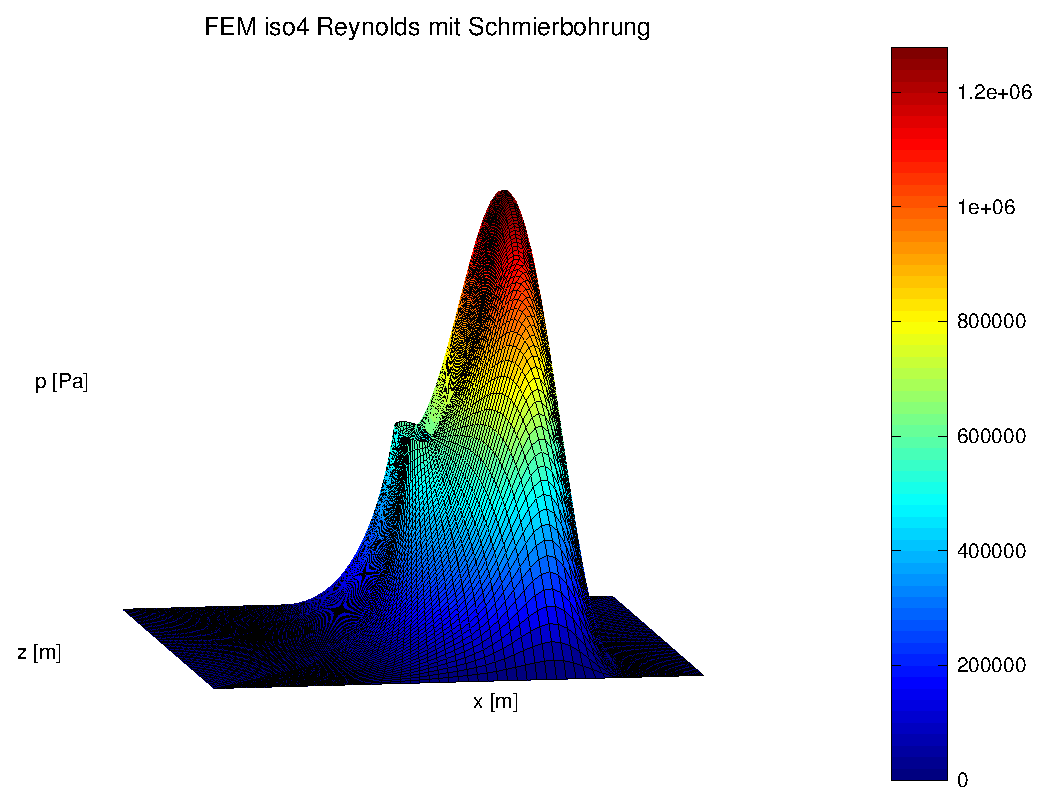
\includegraphics[width=\linewidth]{fig_hfe300}
\caption{Pressure distribution in the bearing with overpressure lubrication through a hole}
\label{fig:hfe_300}
\end{figure}
